\subsection{Results for simultaneous variations of \texorpdfstring{$\kappat$}{kt}, \texorpdfstring{$\kappab$}{kb}, and anomalous point coupling \texorpdfstring{$\cg$}{cg}}
\label{sec:interpretation-results-ktcgkb}


The parametrization of the theoretical predictions for simultaneous variations of $\kappat$ and $\cg$ are implemented into the likelihood as prescribed in Equation~(\ref{eq:likelihood-interpretation}).
% 
The test statistic $q$ is computed over a grid with dimensions $\kappat$ and $\cg$, while the other Higgs boson couplings are fixed at their value expected in the SM.
% 
The 2-dimensional likelihood is shown in Fig.~\ref{fig:ktcg}, under the assumption of branching fractions scaling according to the SM prescription (left) and with the branching ratios implemented as nuisance parameters without any prior constraint (right).


The constraints on the couplings can be factorized into two contributions: one from the shape of the differential distribution, and another from the overall normalization.
% 
Note that the inclusive cross section $\sigma_\text{incl} \sim \left| \kappat^2 + A \cdot \cg^2 \right|$, and the SM in the limit of infinite $\mt$ is given by $(\kappat=0, \cg=1/A)$ (where $A=12$ for the chosen definition of $\cg$~\cite{Grazzini:2016paz}).
% 
Consequently, along the diagonal from $(\kappat=0, \cg=1/A)$ to $(\kappat=1, \cg=0)$, $\sigma_\text{incl}$ is at its SM expected value.
% 
Deviations from this diagonal are thus suppressed when the overall normalization is not profiled in the fit, as can be seen in Fig.~\ref{fig:ktcg} (left).


In Equation~(\ref{eq:interpretation-shape-ktcg}) it was found that the shape of the $\pth$ spectrum via $\ggh$ depends only on the ratio $\kappat/\cg$.
% 
This is clearly visible in Fig.~\ref{fig:ktcg} (right), where the constraints are posed mostly on the ratio $\kappat / \cg$, and in Fig.~\ref{fig:ktcg} (left), where the constraint \emph{along} the diagonal comes from the shape of the $\ggh$ spectrum.
% 
Applying the logic of Equation~(\ref{eq:interpretation-shape-ktcg}) analogously on the other production modes reveals that here the constraints do not manifest themselves purely in the ratio.
% 
This explains why transformations such as Equation~(\ref{eq:interpretation-ktcg-transform}) do not hold at small values of the couplings (as can be seen in Fig.~\ref{fig:ktcg} (right)), where the $\ggh$ production mode is no longer dominant over the others.
% 
In the case of unconstrained branching fractions, there is an overall symmetry under $(\kappat,\,\cg) \, \to \, (-\kappat,\,-\cg)$, hence the two symmetric sets of contours in Fig.~\ref{fig:ktcg} (right).
% 
In the case of coupling-dependent branching fractions, this symmetry is broken by a linear term in $\kappat$ in $\BRgamgam$.
% 
A final noteworthy feature about Fig.~\ref{fig:ktcg} (right), is that seemingly the combination constrains the ratio $\kappat / \cg$ less than the $\hgg$ channel by itself; this is a feature of the observed data that is not seen in expected fits.
% 
These features may arise when the combination cancels out opposite deviations in the individual channels.


\begin{figure}[hbtp]
  \begin{center}
    \ifbool{draftmode}{
        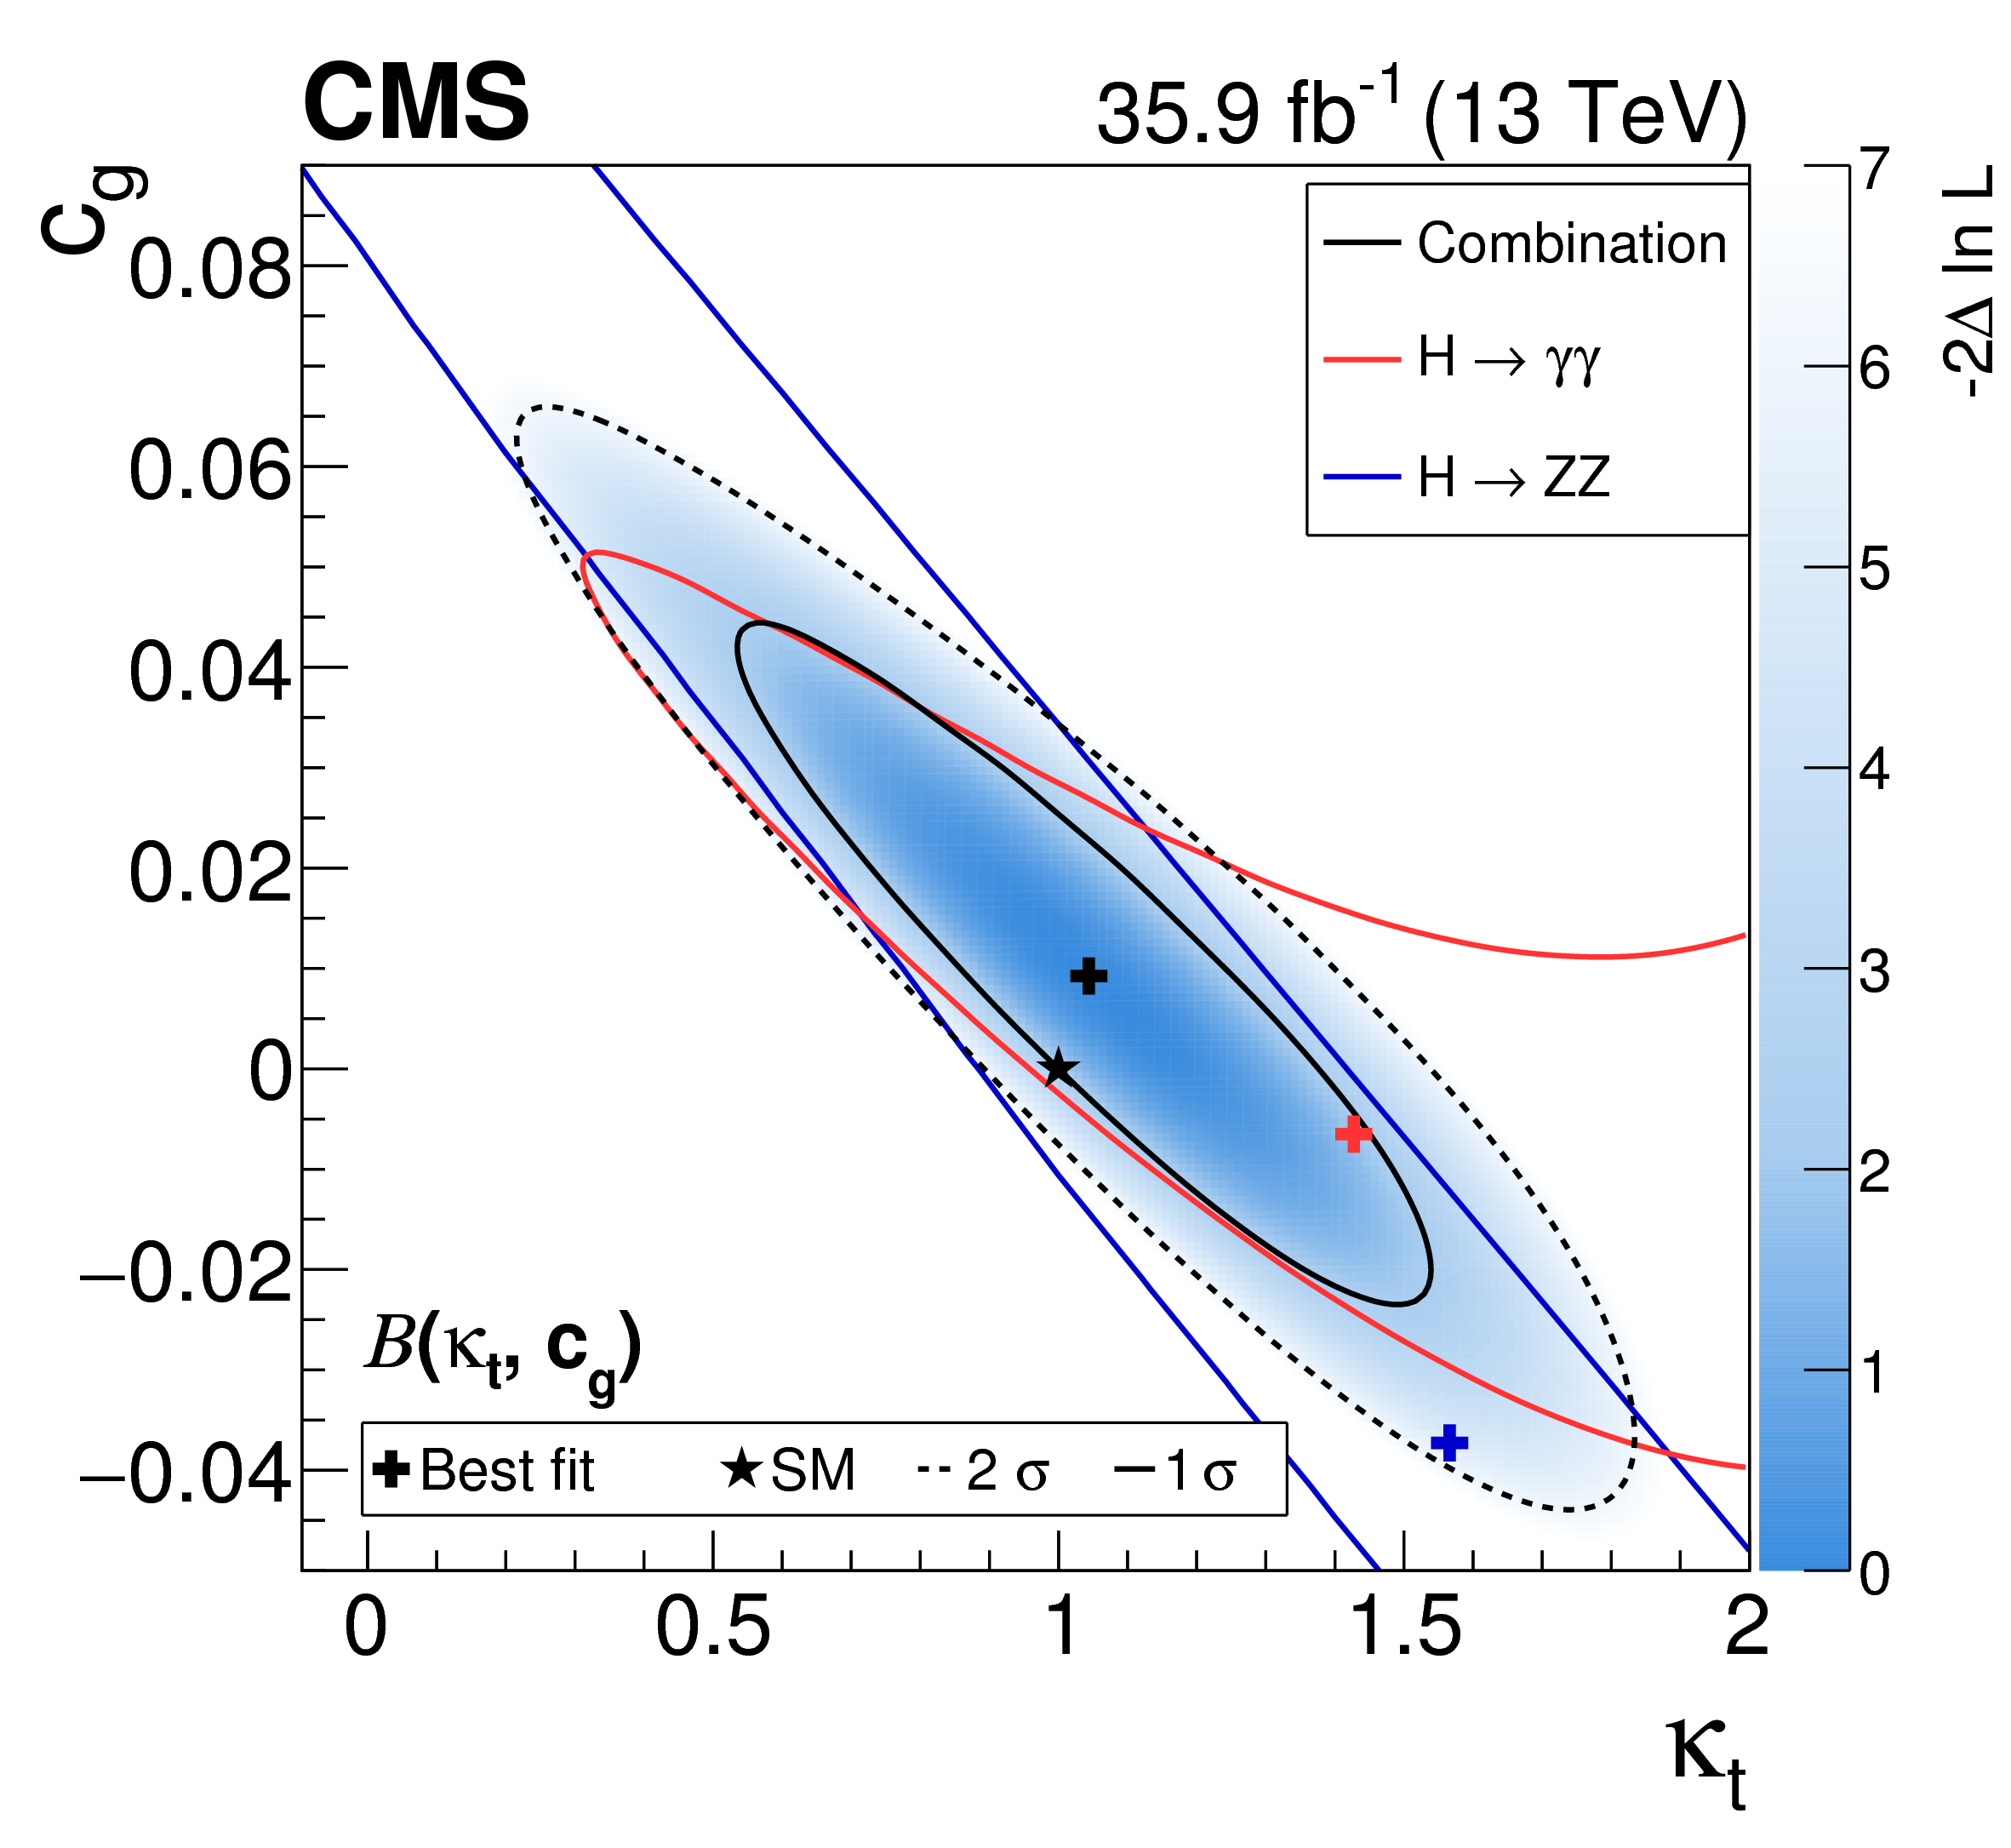
\includegraphics[width=0.49\linewidth]{img/interpretation/multicont_ktcg_couplingdependentBRs.png}
        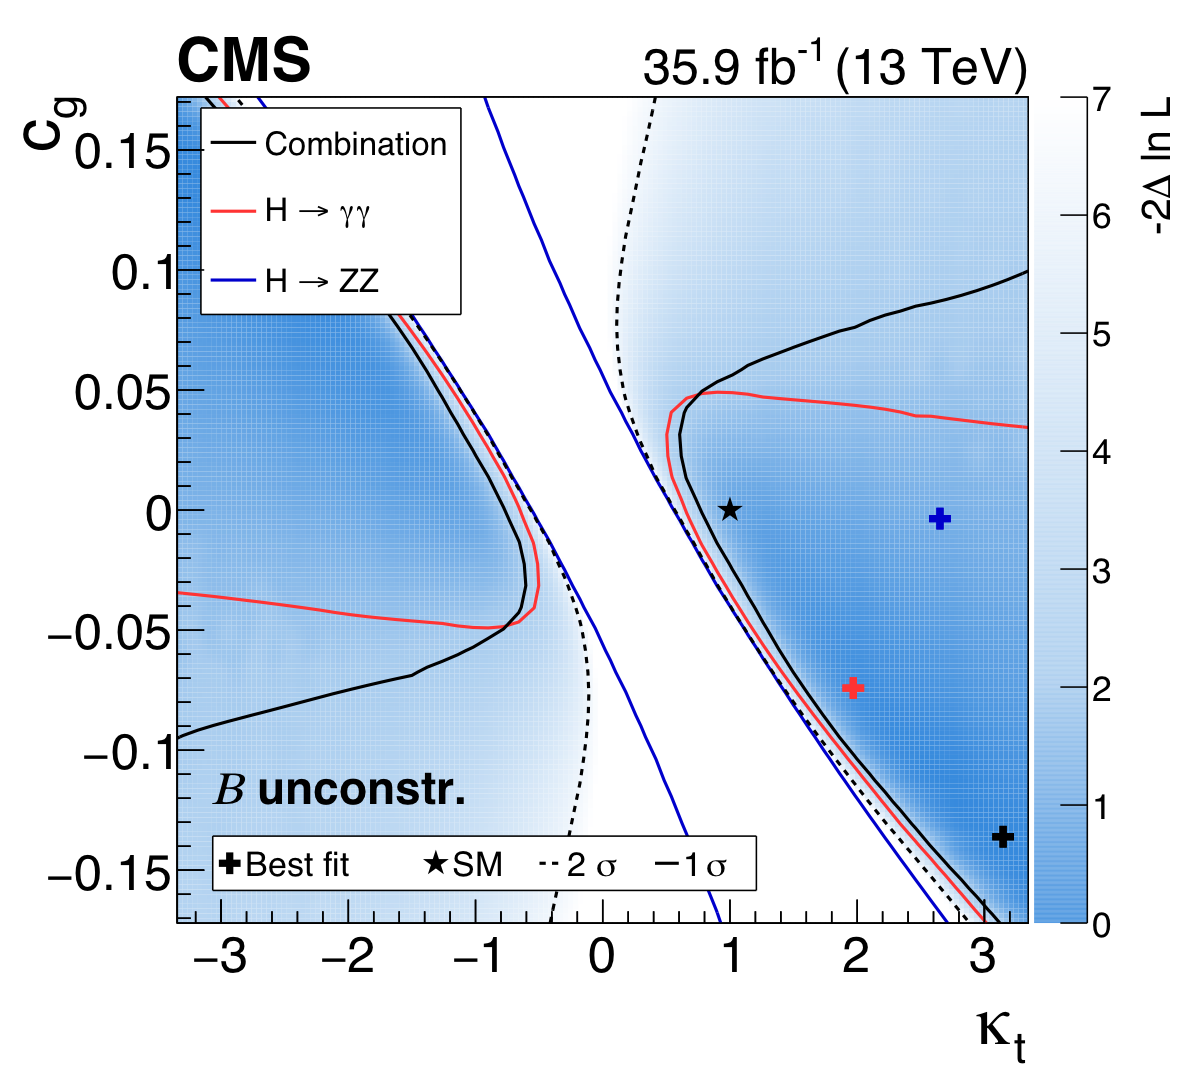
\includegraphics[width=0.49\linewidth]{img/interpretation/multicont_ktcg_floatingBRs.png}
        }{
        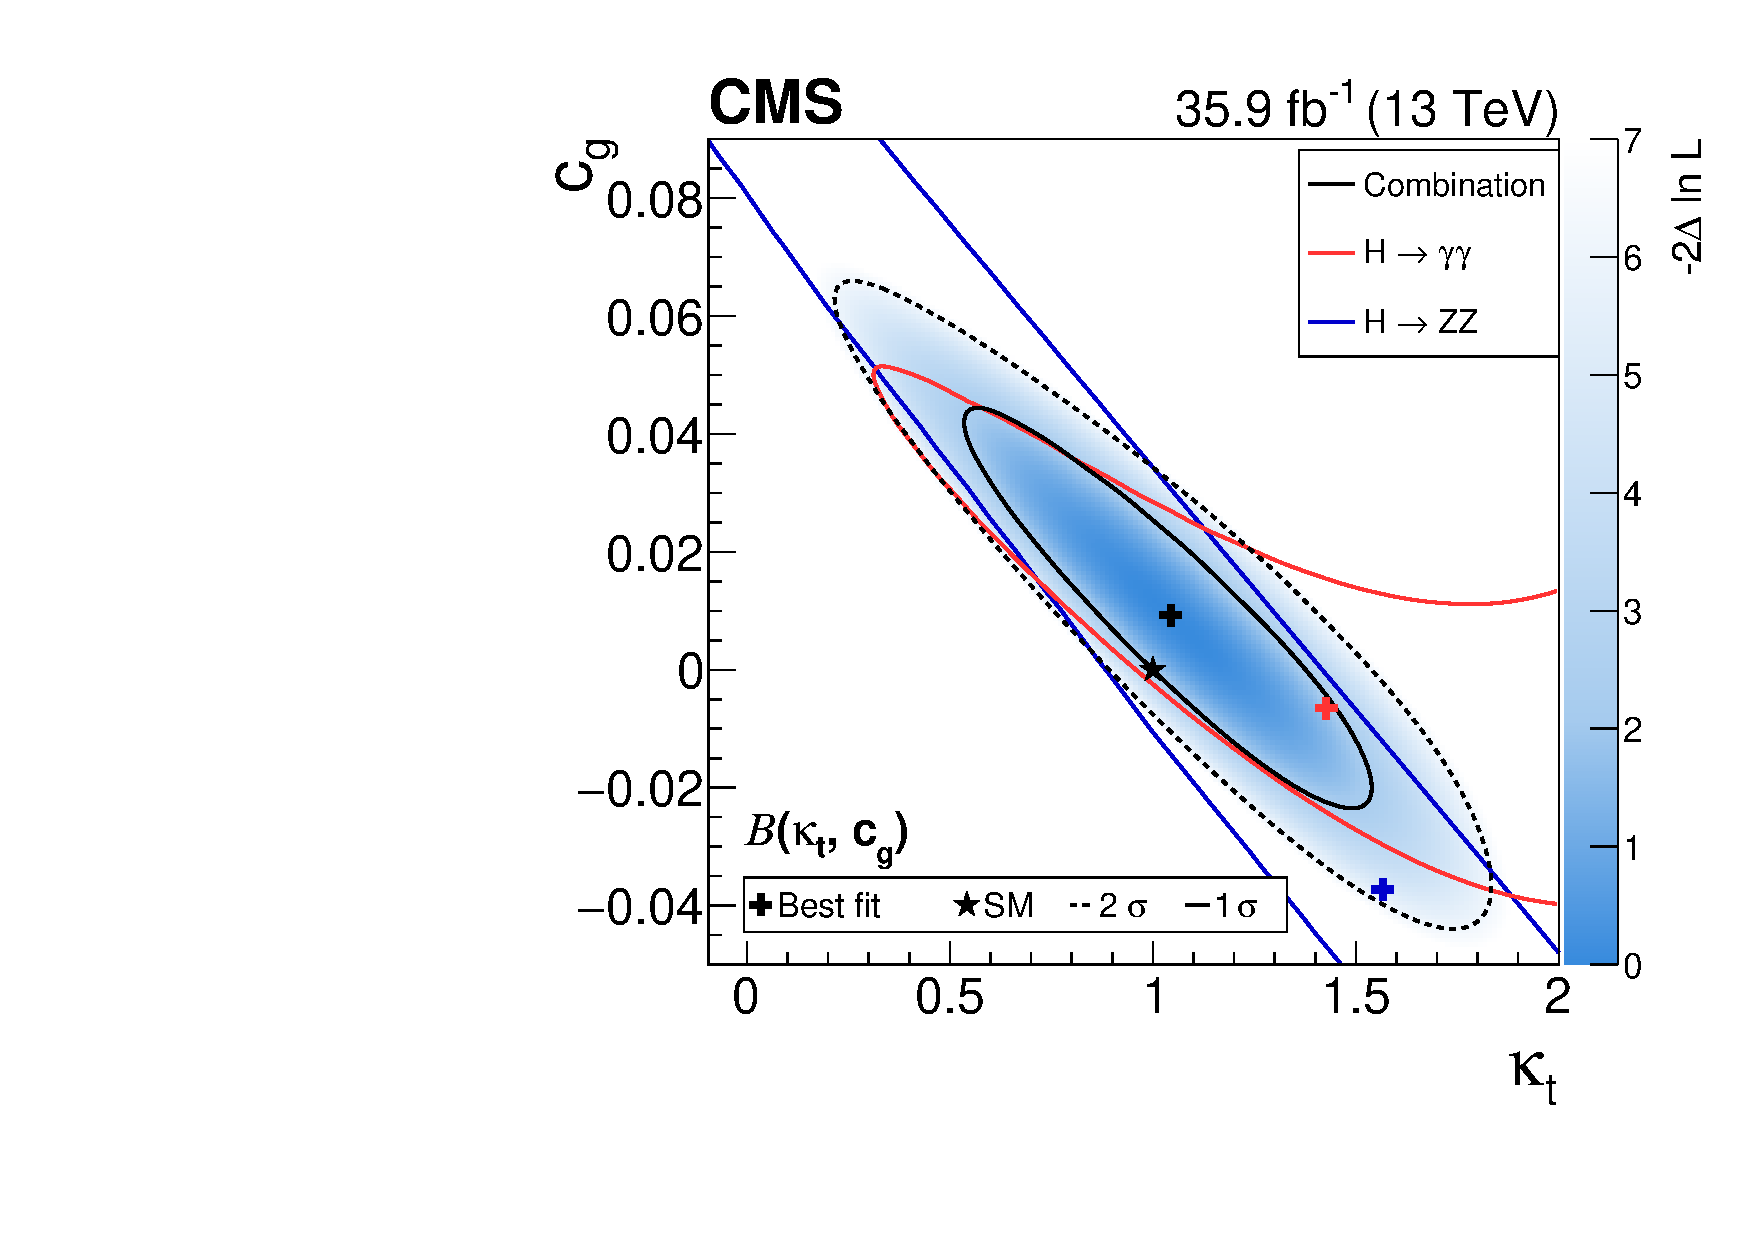
\includegraphics[width=0.49\linewidth]{img/interpretation/multicont_ktcg_couplingdependentBRs.pdf}
        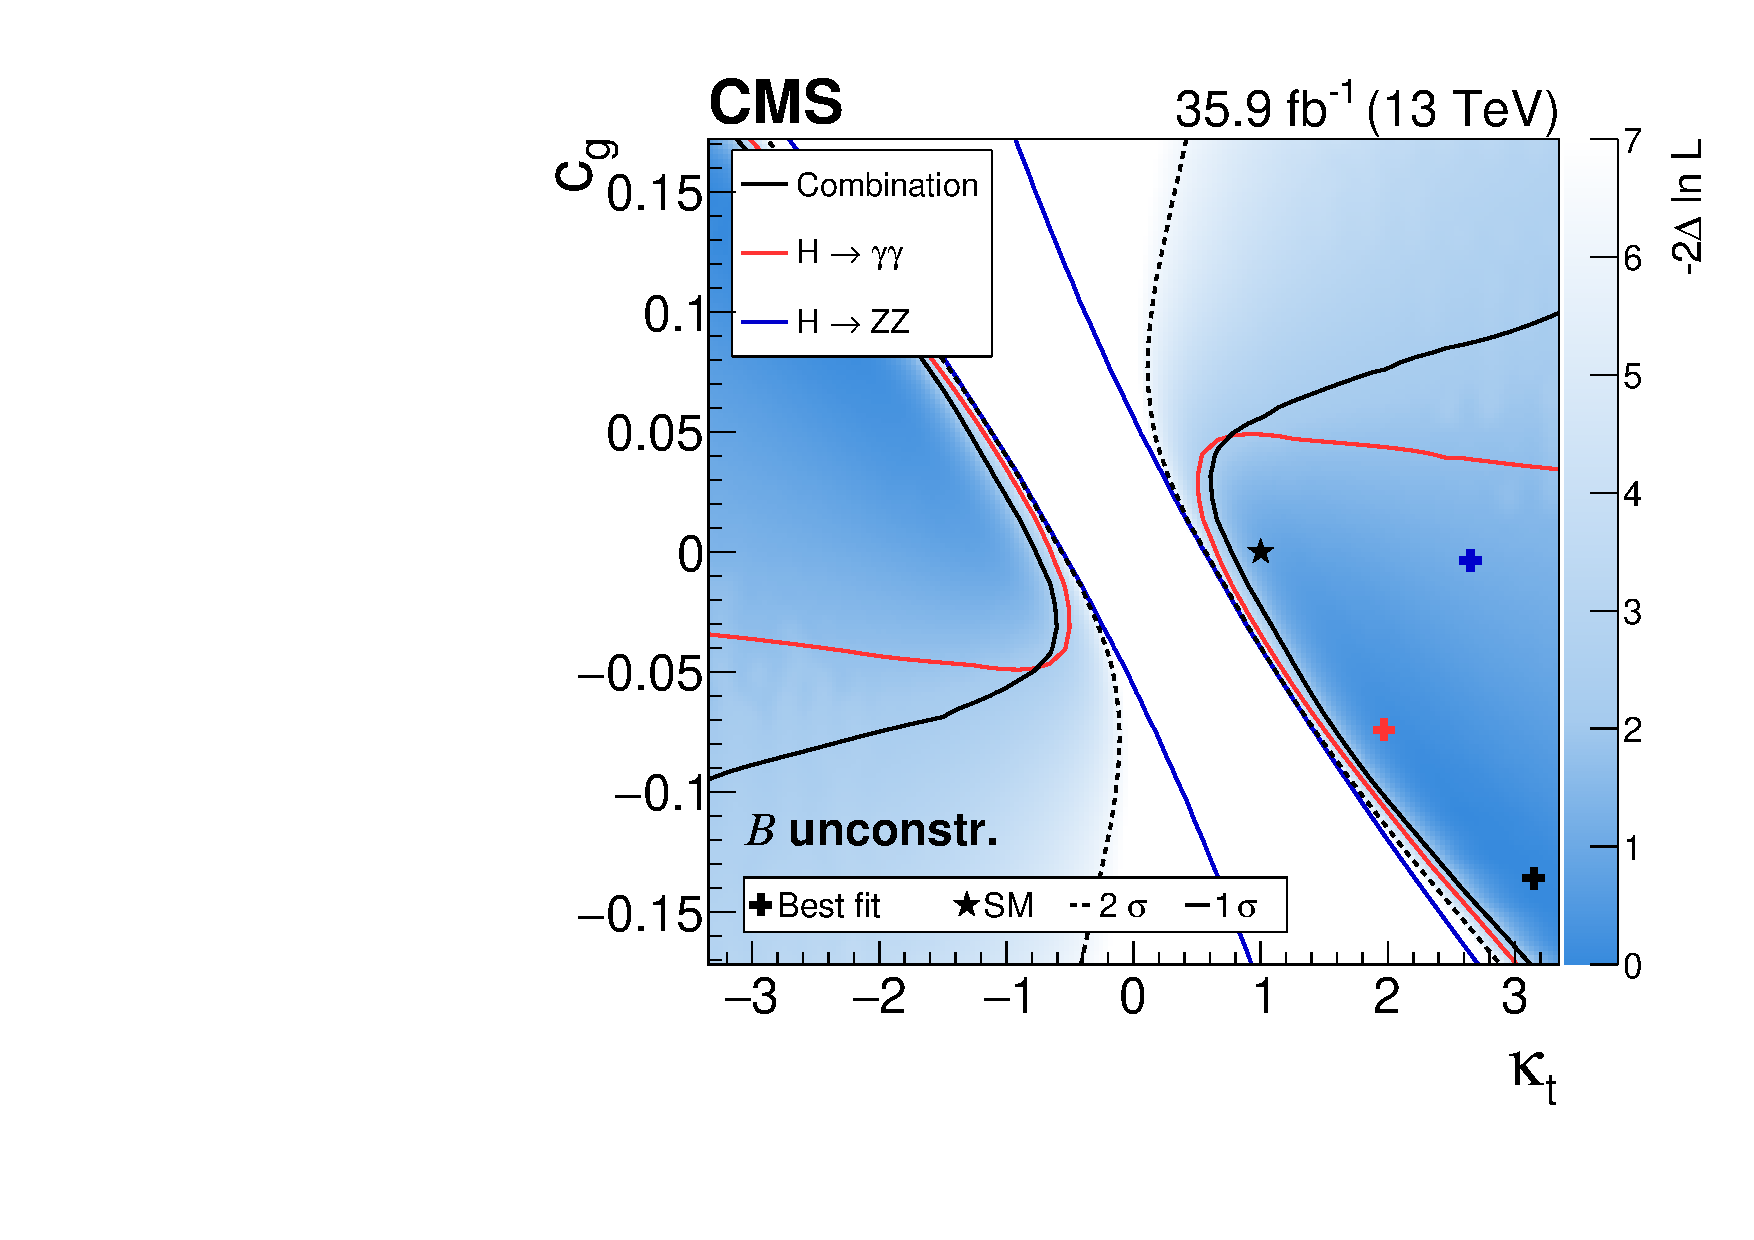
\includegraphics[width=0.49\linewidth]{img/interpretation/multicont_ktcg_floatingBRs.pdf}        
        }
    % 
    \caption{
        Simultaneous fit to data for $\kappat$ and $\cg$, assuming a coupling dependence of the branching fractions (left) and the branching fractions implemented as nuisance parameters with no prior constraint (right).
        % 
        The one standard deviation contour is drawn for the combination ($\hgg$, $\hzz$, and $\hbb$), the $\hgg$ channel, and the $\hzz$ channel in black, red, and blue, respectively.
        % 
        For the combination the two standard deviation contour is drawn as a black dashed line, and the shading indicates the negative log-likelihood, with the scale shown on the right hand side of the plots.
        }
    \label{fig:ktcg}
  \end{center}
\end{figure}


As an illustration, Fig.~\ref{fig:ktcg-points} shows four examples of the $\pth$ spectra for sets of $(\kappat, \cg)$ that are excluded by exactly 2-standard-deviations.
% 
As expected, the tail of the measurement drives the allowed shape of the $\pth$ spectrum, while the lower $\pth$ region provides the constraint due to the overall normalization.


\begin{figure}[hbtp]
  \begin{center}
    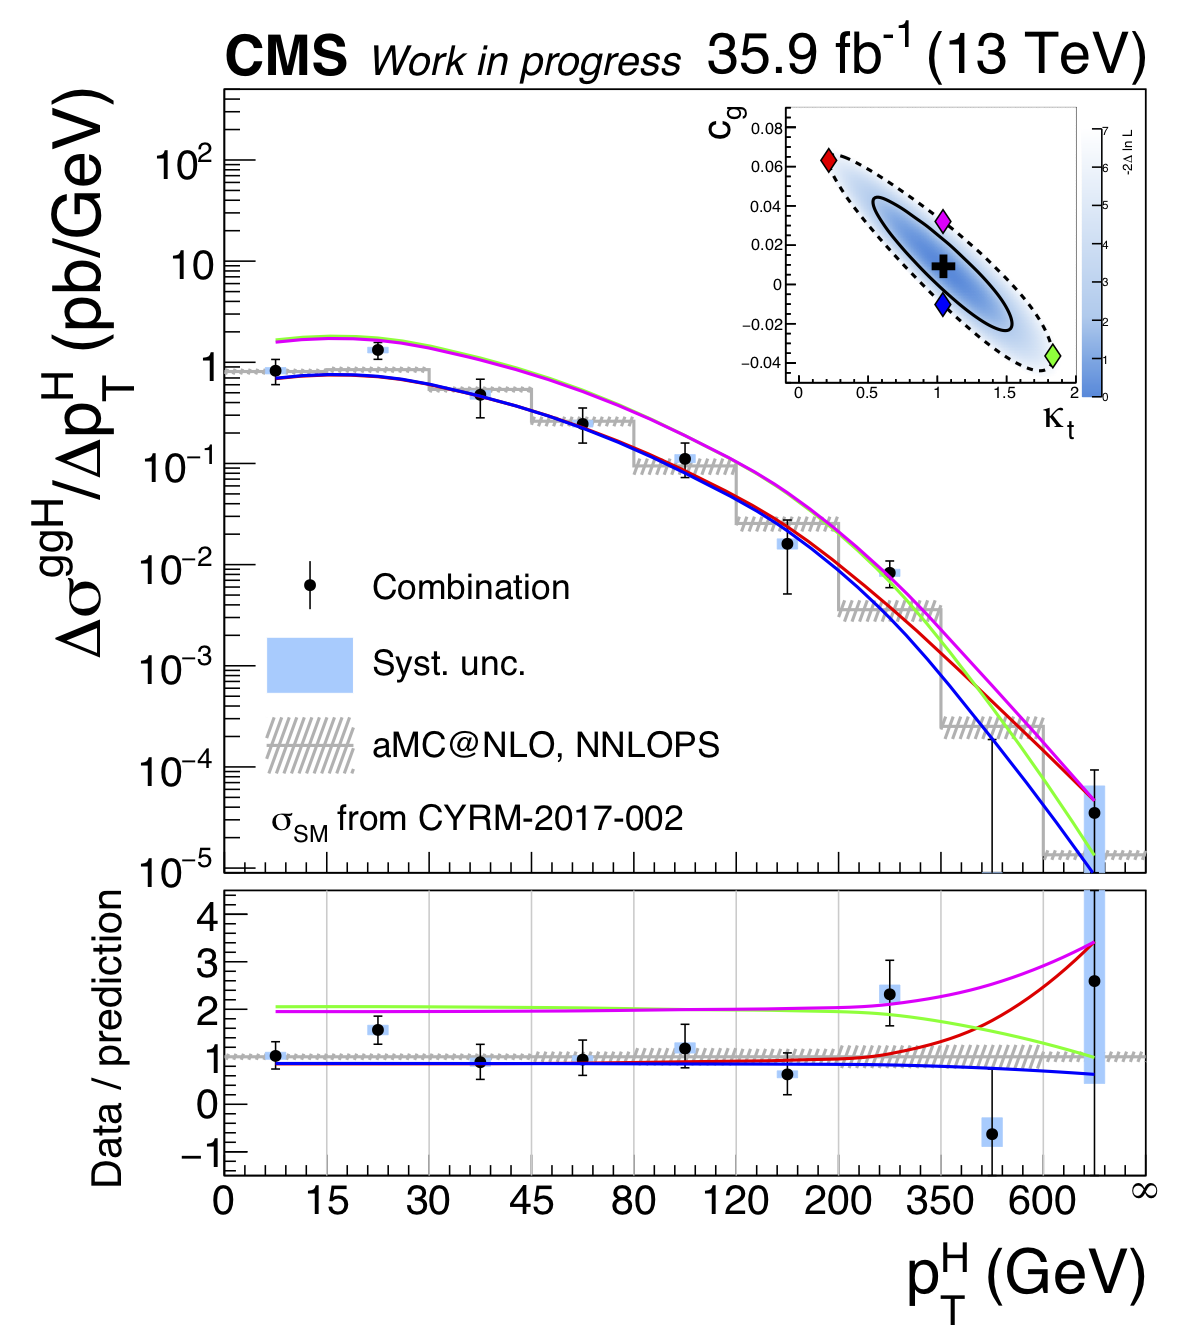
\includegraphics[width=0.55\linewidth]{img/interpretation/spectra_pth_ggH_withmulticont.png}
    % 
    \caption{
        The combined $\pth$ spectrum for the $\ggh$ production mode, along with theoretical predictions for several $(\kappat, \cg)$ points on the 2-standard-deviation contour.
        % 
        The diamonds in the panel in the upper right corner correspond to the theoretical $\pth$ spectra of the same color.
        }
    \label{fig:ktcg-points}
  \end{center}
\end{figure}


It is noteworthy that in both scenarios the SM in the infinite $\mt$ limit is excluded by $4.4$ and $2.2$ standard deviations for the coupling-dependent branching fractions and the unconstrained branching fractions, respectively.
% 
This poses experimental evidence for the existence of the gluon fusion production loop, rather than a direct coupling of the Higgs boson to the gluon field.



% ____________________________________________________________________________
% kt/kb

A fit of the parametrization of the same model, but now with $\kappat$ and $\kappab$ as the fitted parameters, is shown in Fig.~\ref{fig:ktkb} (left), for the fit with the branching fractions implemented as functions of the couplings.
% 
The likelihood is driven by constraints on the inclusive cross section times the branching fractions, $\sigma_\text{incl} \times \BRgamgam$ and $\sigma_\text{incl} \times \BRZZ$.
% 
The dependence of the cross section on the couplings is quadratic by construction.
% 
As in the case of variations of $\kappat$ and $\cg$, $\BRgamgam$ contains a linear term in $\kappat$, hence the likelihood in the $\hgg$ channel and in the combination is not symmetric under $(\kappat,\,\kappab) \, \to \, (-\kappat,\,-\kappab)$, unlike the result in the $\hzz$ channel.
% 
Deviations from the circular band in the $\hgg$ channel are excluded mostly due to the fact that $\sigma_\text{incl} \times \BRgamgam$ would then deviate too much from the observed data.
% 
At simultaneously low values of $\kappat$ and $\kappab$, $\BRgamgam$ becomes very large, explaining the `gap' in the circular band.


In Fig.~\ref{fig:ktkb} (right) the branching fractions are unconstrained, thus fitting only the shape of the parametrization to data.
% 
As the linear dependence on $\kappat$ disappears, the likelihood becomes symmetric under $(\kappat,\,\kappab) \, \to \, (-\kappat,\,-\kappab)$ for all decay channels.
% 
Applying Equation~(\ref{eq:interpretation-shape-ktcg}) analogously on the parametrization of $\ggh$ for variations of $\kappat$ and $\kappab$ reveals that also here the shape of the differential distribution depends solely on the slope $\kappab/\kappat$, explaining the invariance under transformations like $(\kappat, \kappab) \to (c \cdot \kappat, c \cdot \kappab)$ for larger values of the couplings.



\begin{figure}[hbtp]
  \begin{center}
    \ifbool{draftmode}{
        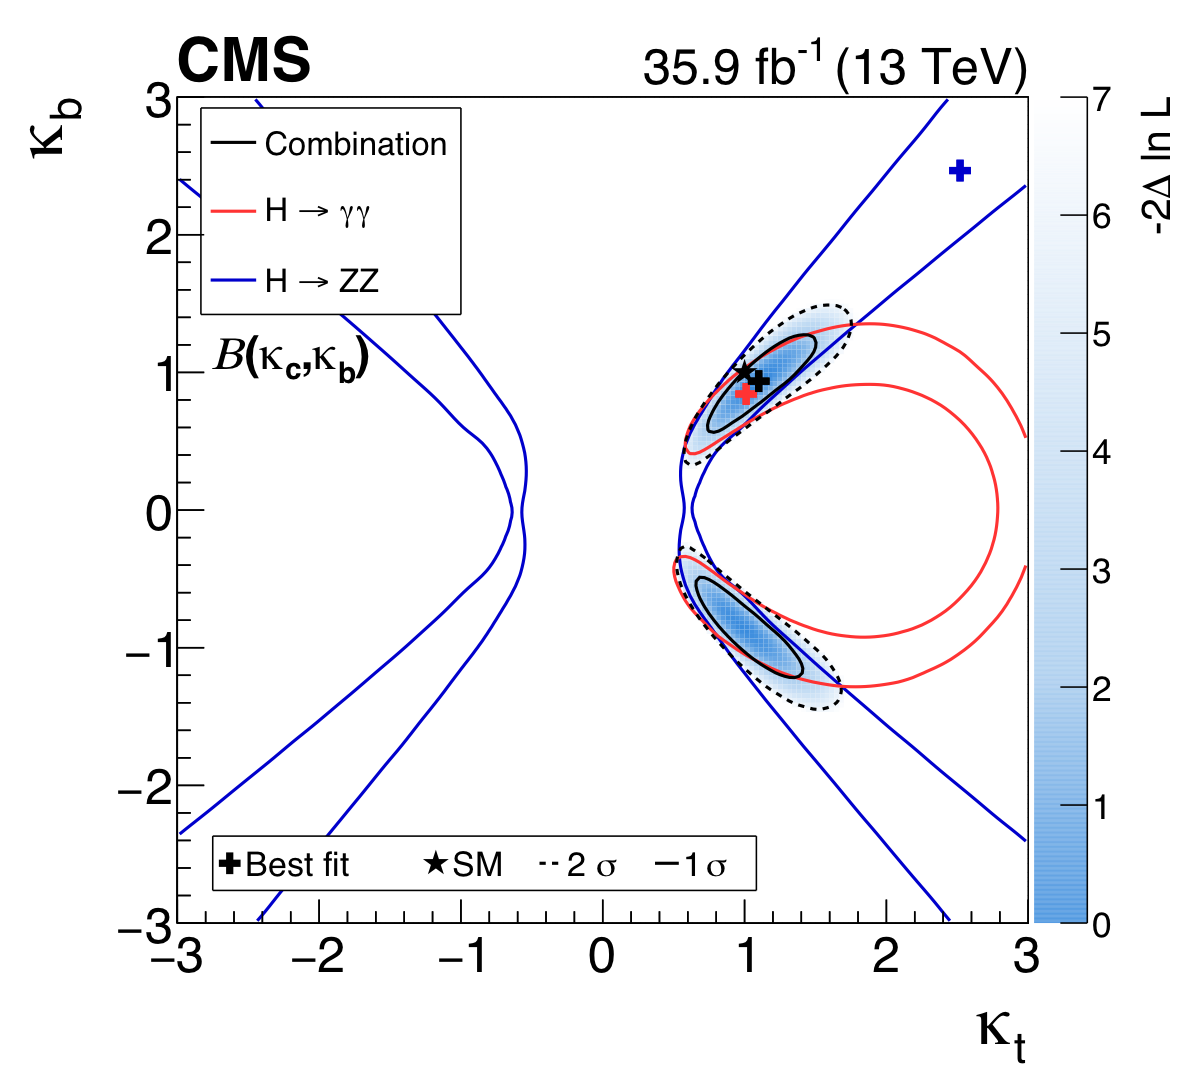
\includegraphics[width=0.49\linewidth]{img/interpretation/multicont_ktkb_couplingdependentBRs.png}
        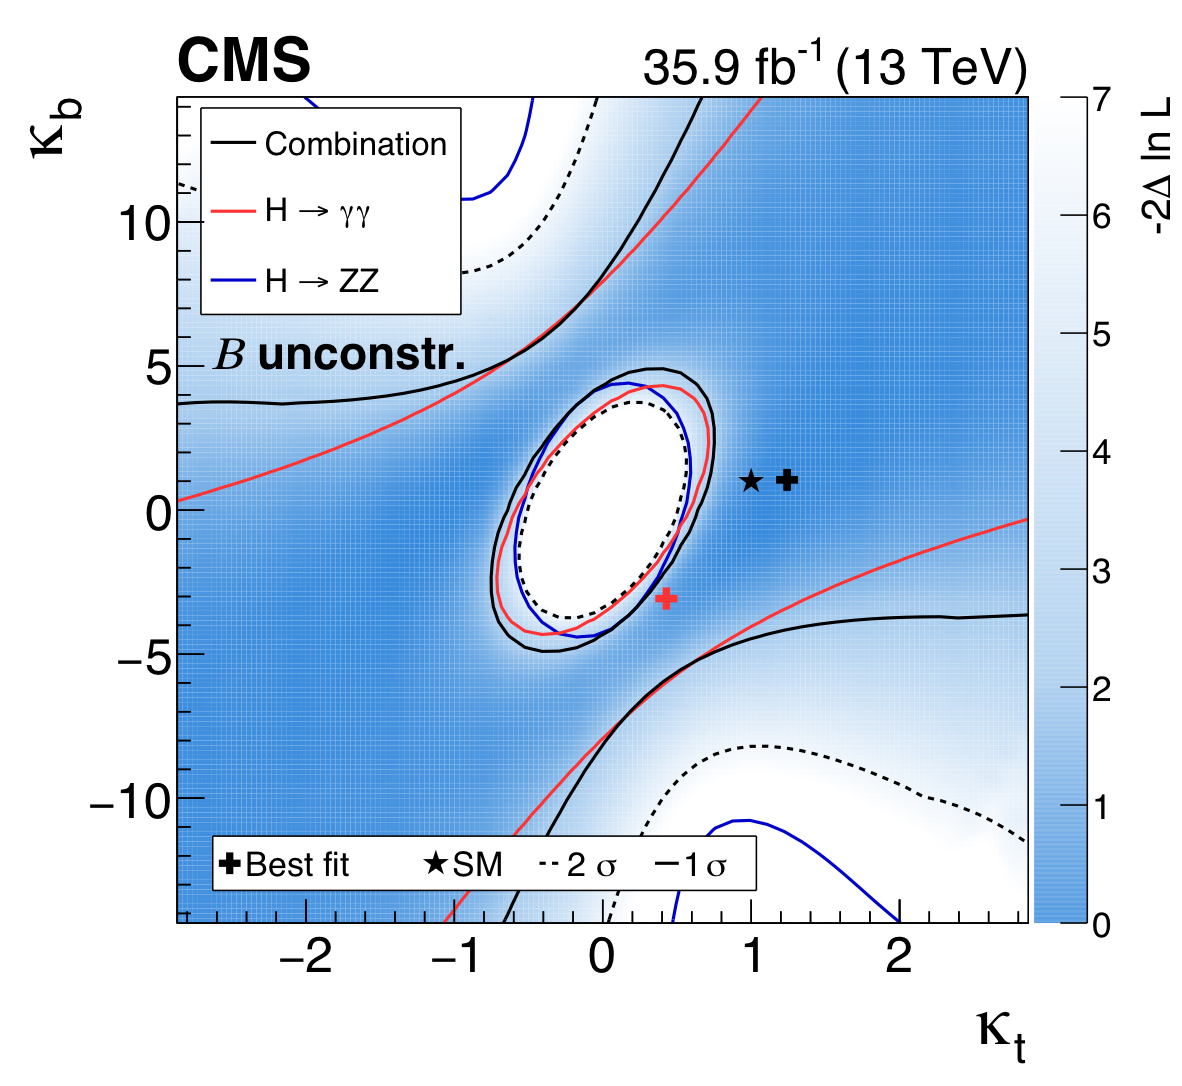
\includegraphics[width=0.49\linewidth]{img/interpretation/multicont_ktkb_floatingBRs.png}
        }{
        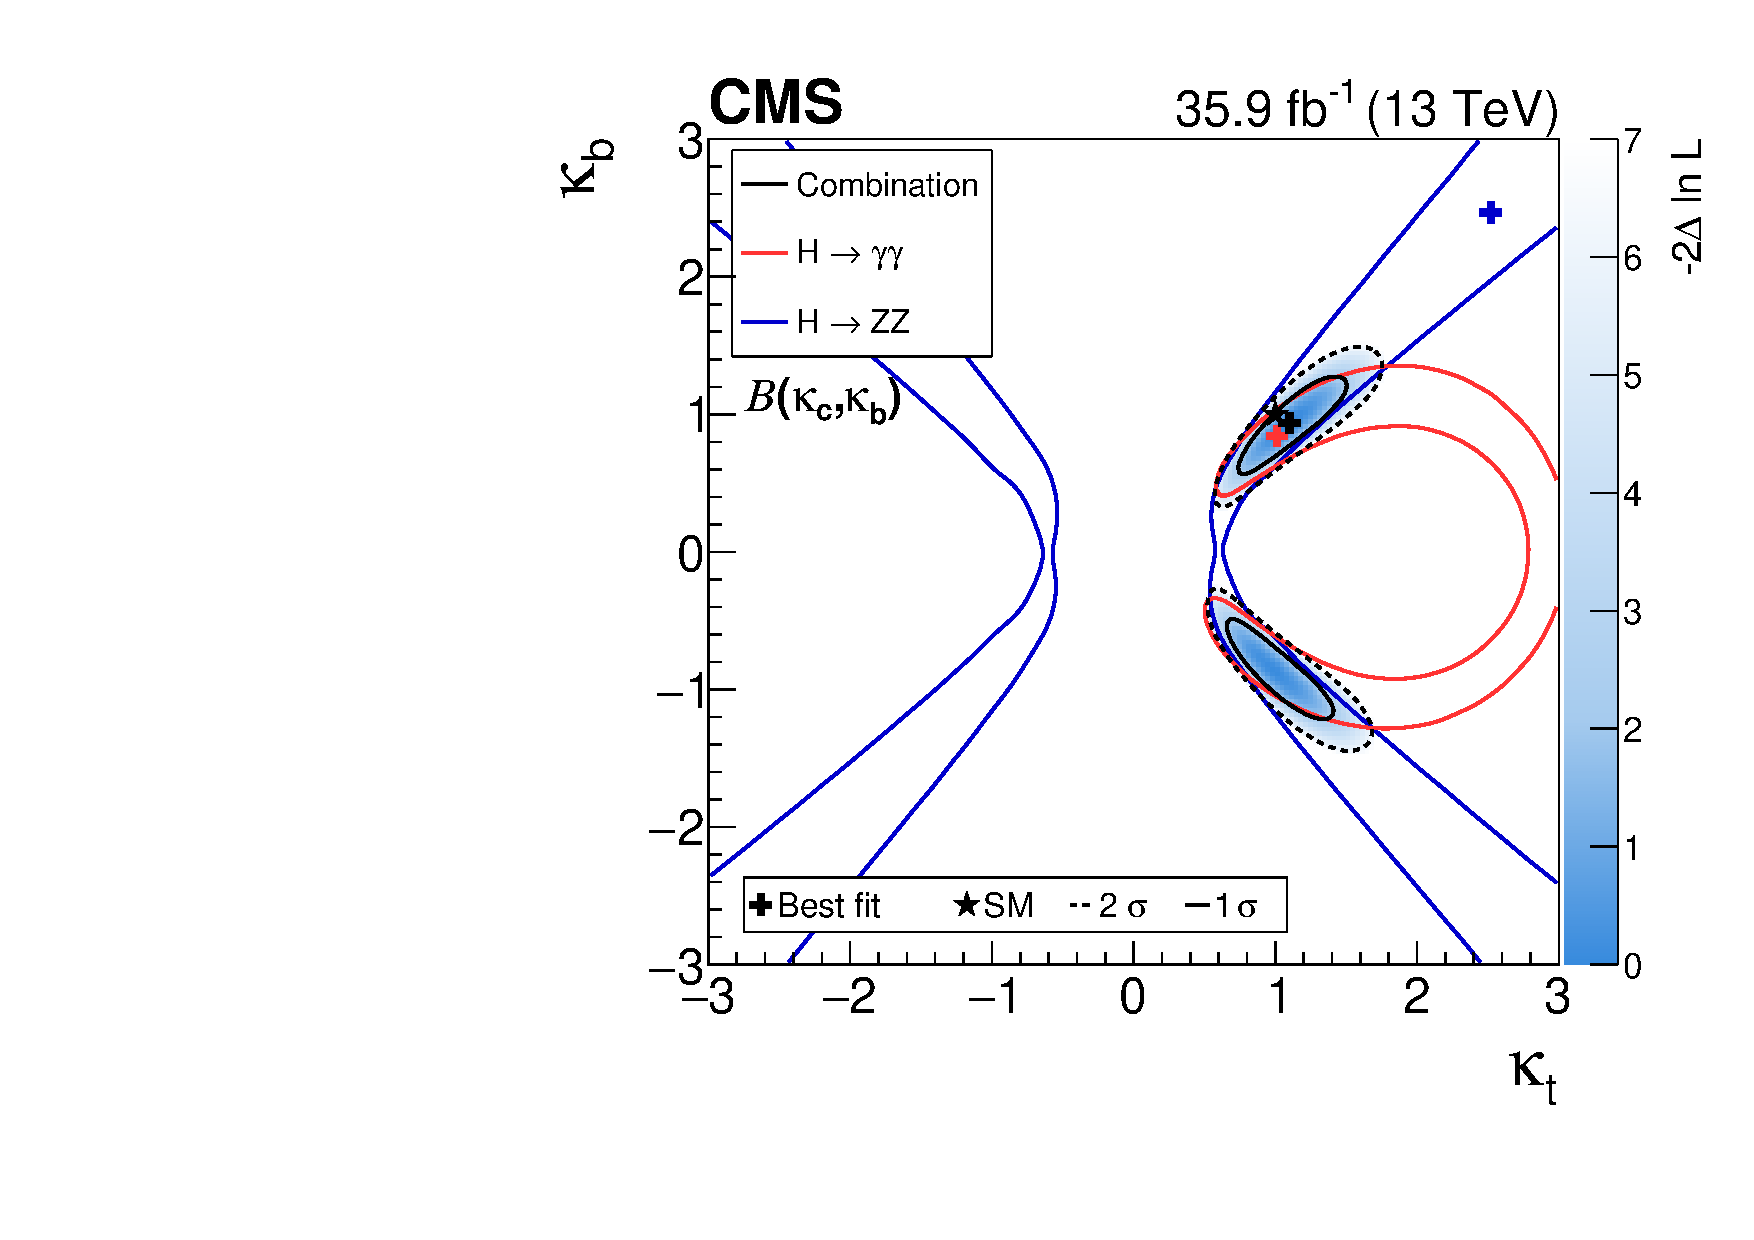
\includegraphics[width=0.49\linewidth]{img/interpretation/multicont_ktkb_couplingdependentBRs.pdf}
        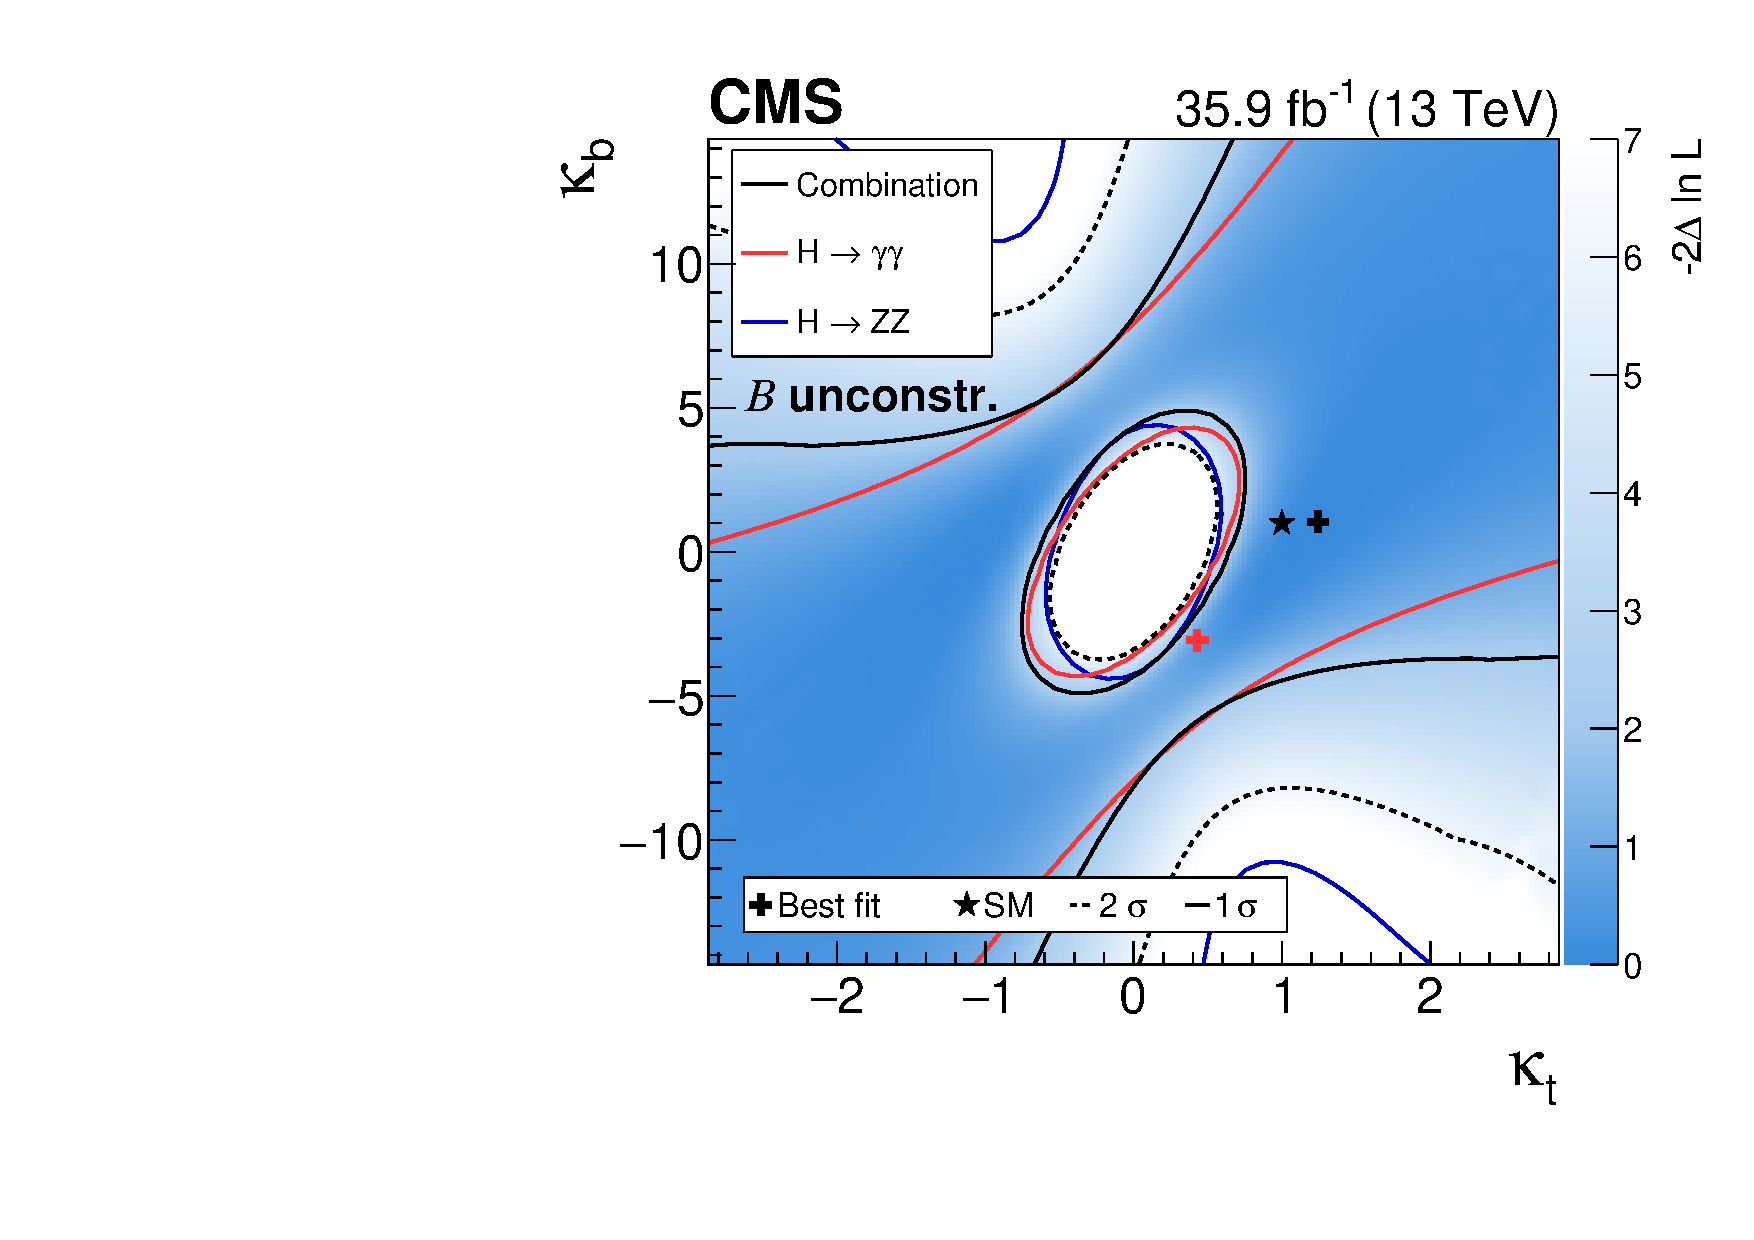
\includegraphics[width=0.49\linewidth]{img/interpretation/multicont_ktkb_floatingBRs.pdf}        
        }
    % 
    \caption{
        Simultaneous fit to data for $\kappat$ and $\kappab$, assuming a coupling dependence of the branching fractions (left) and the branching fractions implemented as nuisance parameters with no prior constraint (right).
        % 
        The one standard deviation contour is drawn for the combination ($\hgg$, $\hzz$, and $\hbb$), the $\hgg$ channel, and the $\hzz$ channel in black, red, and blue, respectively.
        % 
        For the combination the two standard deviation contour is drawn as a black dashed line, and the shading indicates the negative log-likelihood, with the scale shown on the right hand side of the plots.
        }
    \label{fig:ktkb}
  \end{center}
\end{figure}


% ____________________________________________________________________________
\subsection{Results for simultaneous variations of \texorpdfstring{$\kappab$}{kb} and \texorpdfstring{$\kappac$}{kc}}
\label{sec:interpretation-results-kbkc}


Analogously to Section~\ref{sec:interpretation-results-ktcgkb}, the theoretical predictions for simultaneous variations of $\kappab$ and $\kappac$ are parametrized and fitted to data.
% 
The fit with the branching fractions implemented as functions of the couplings is shown in Fig.~\ref{fig:kbkc} (left), and the one with the branching fractions implemented as unconstrained nuisance parameters in Fig.~\ref{fig:kbkc} (right).


\begin{figure}[hbtp]
  \begin{center}
    \ifbool{draftmode}{
        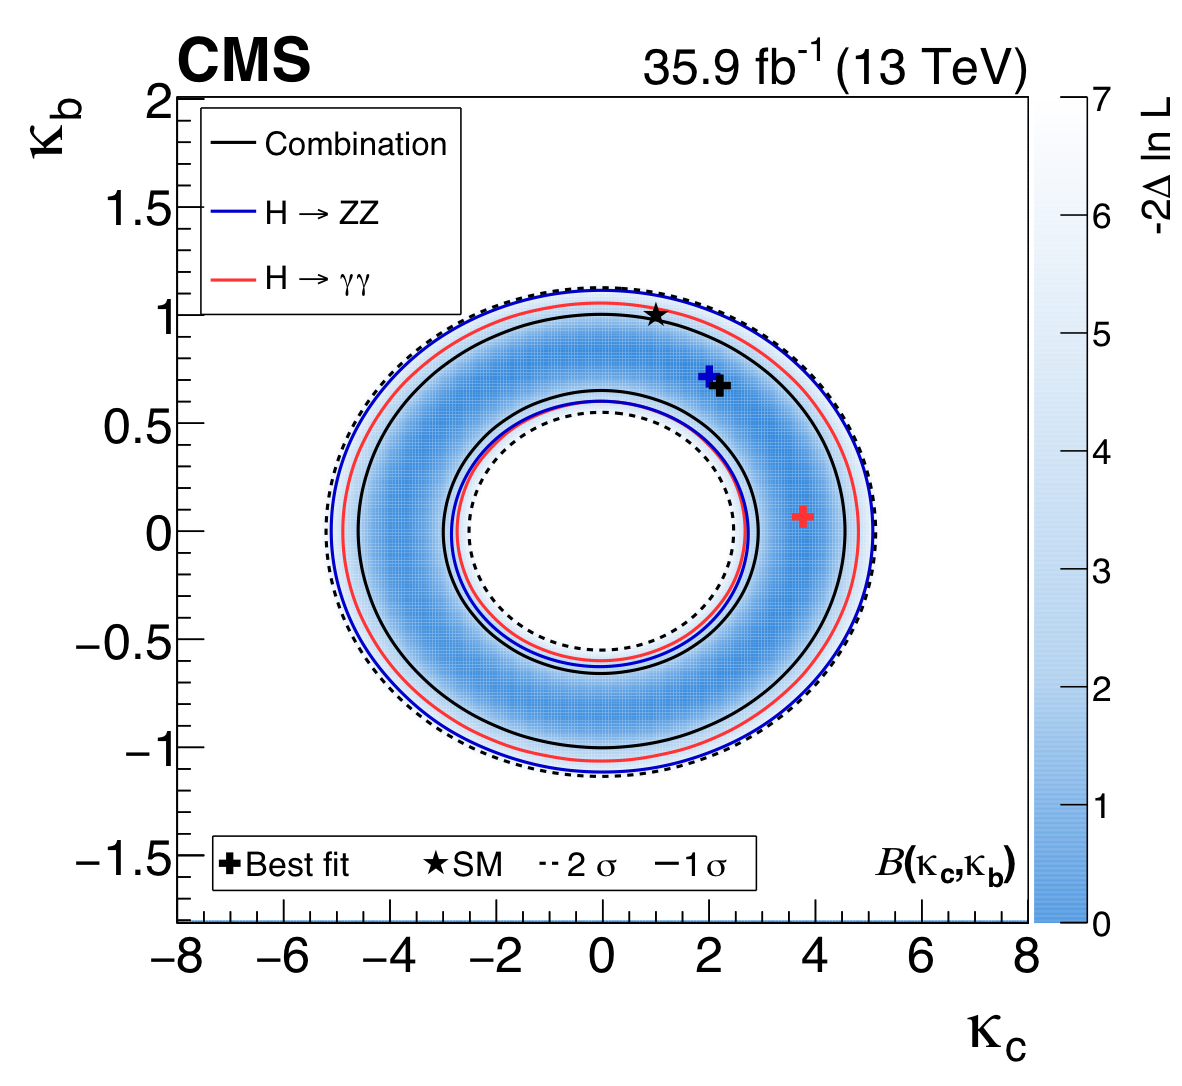
\includegraphics[width=0.49\linewidth]{img/interpretation/multicont_Yukawa_couplingdependentBRs.png}
        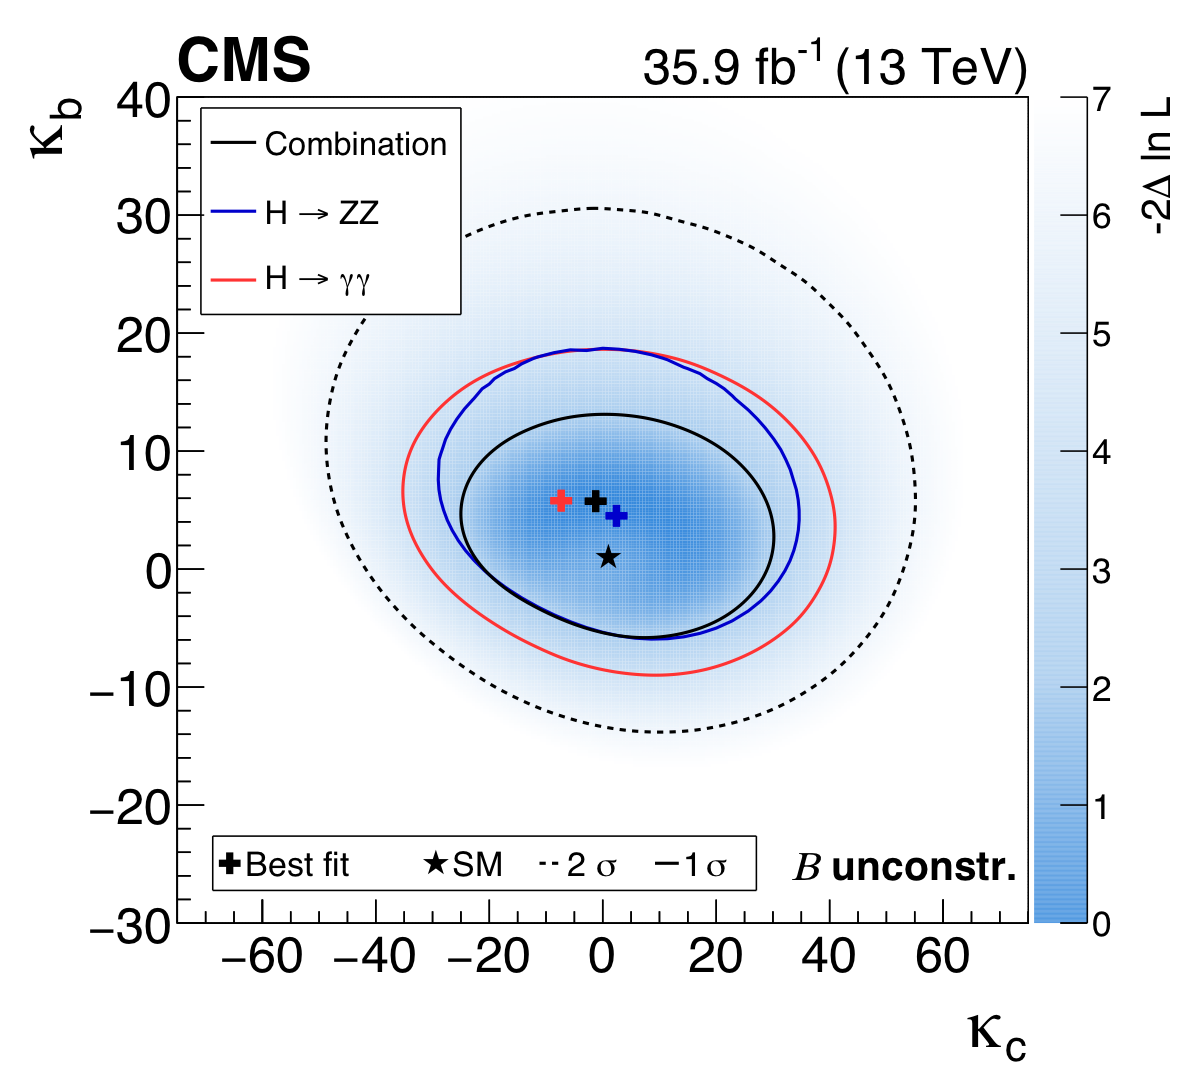
\includegraphics[width=0.49\linewidth]{img/interpretation/multicont_Yukawa_floatingBRs.png}
        }{
        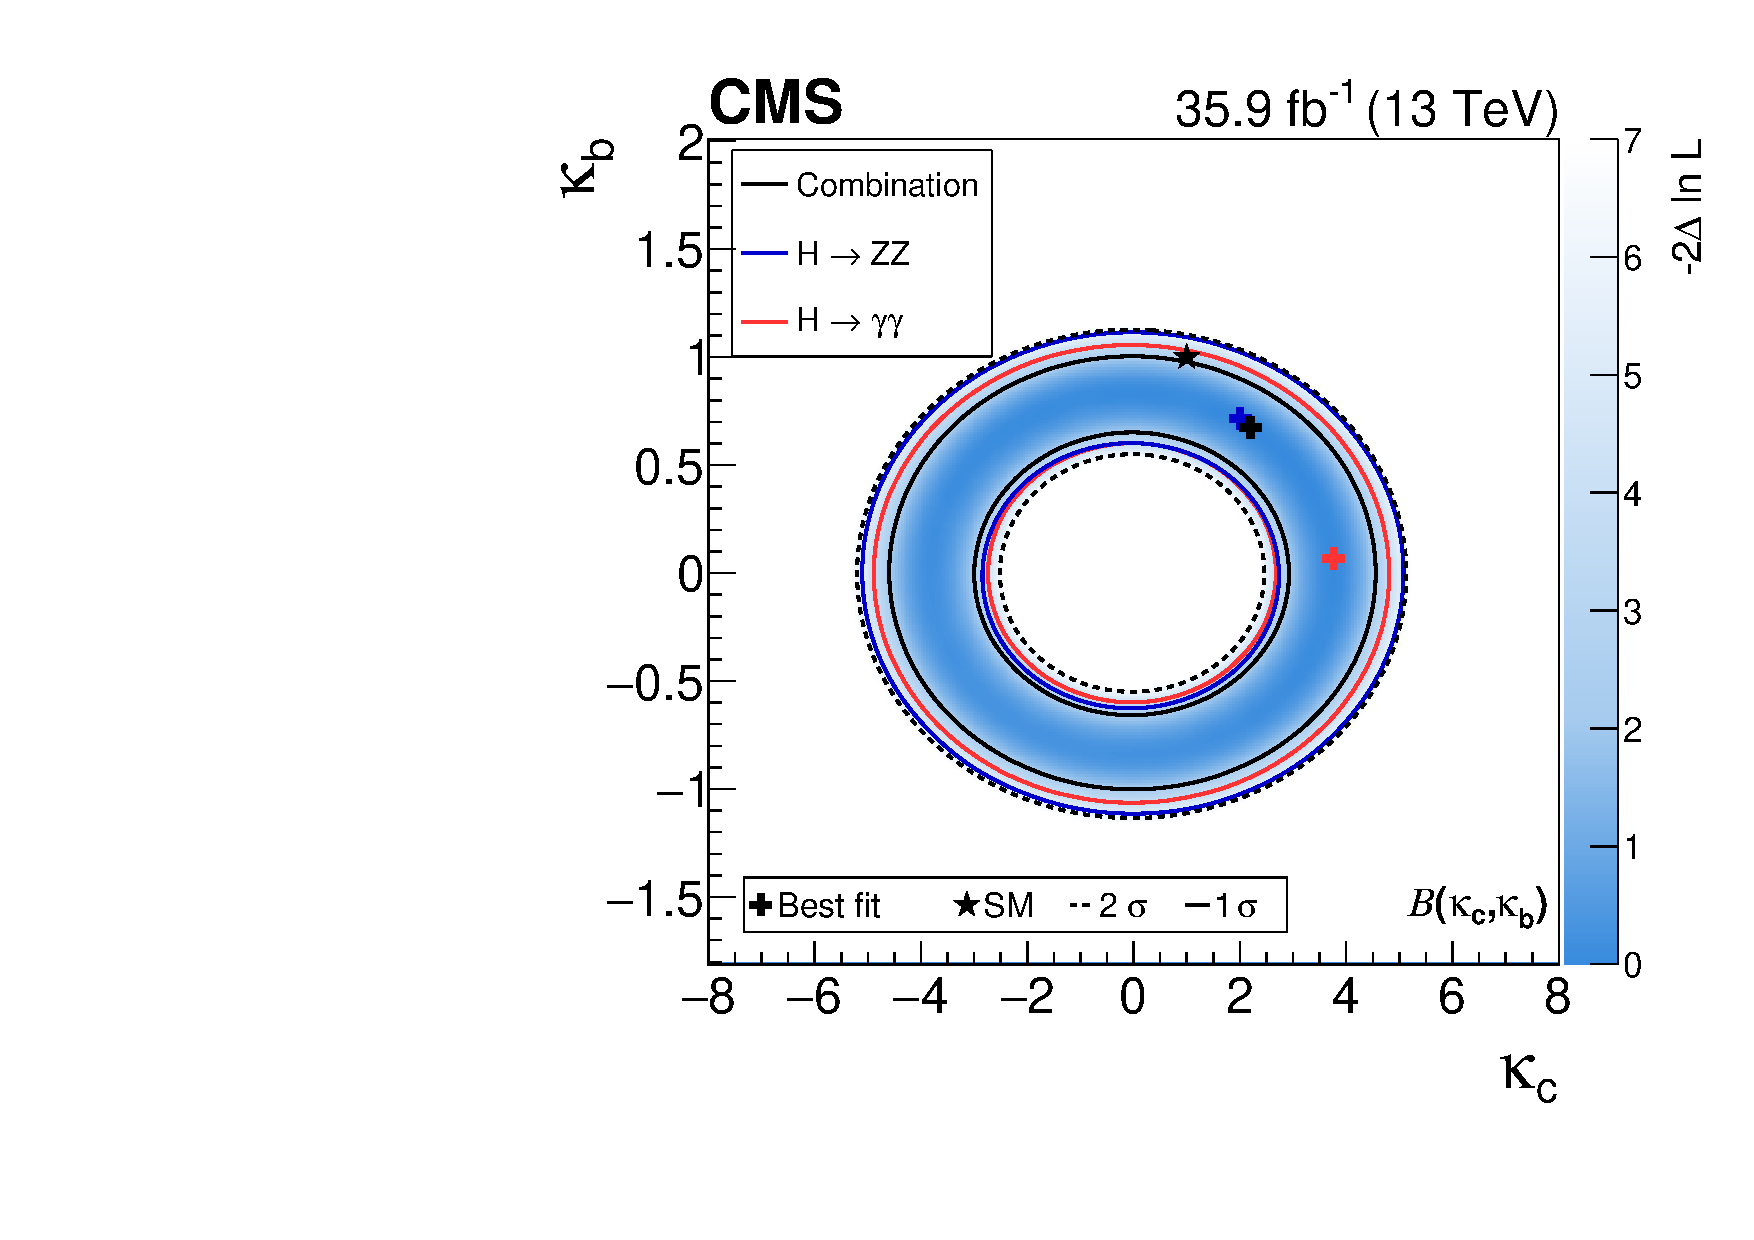
\includegraphics[width=0.49\linewidth]{img/interpretation/multicont_Yukawa_couplingdependentBRs.pdf}
        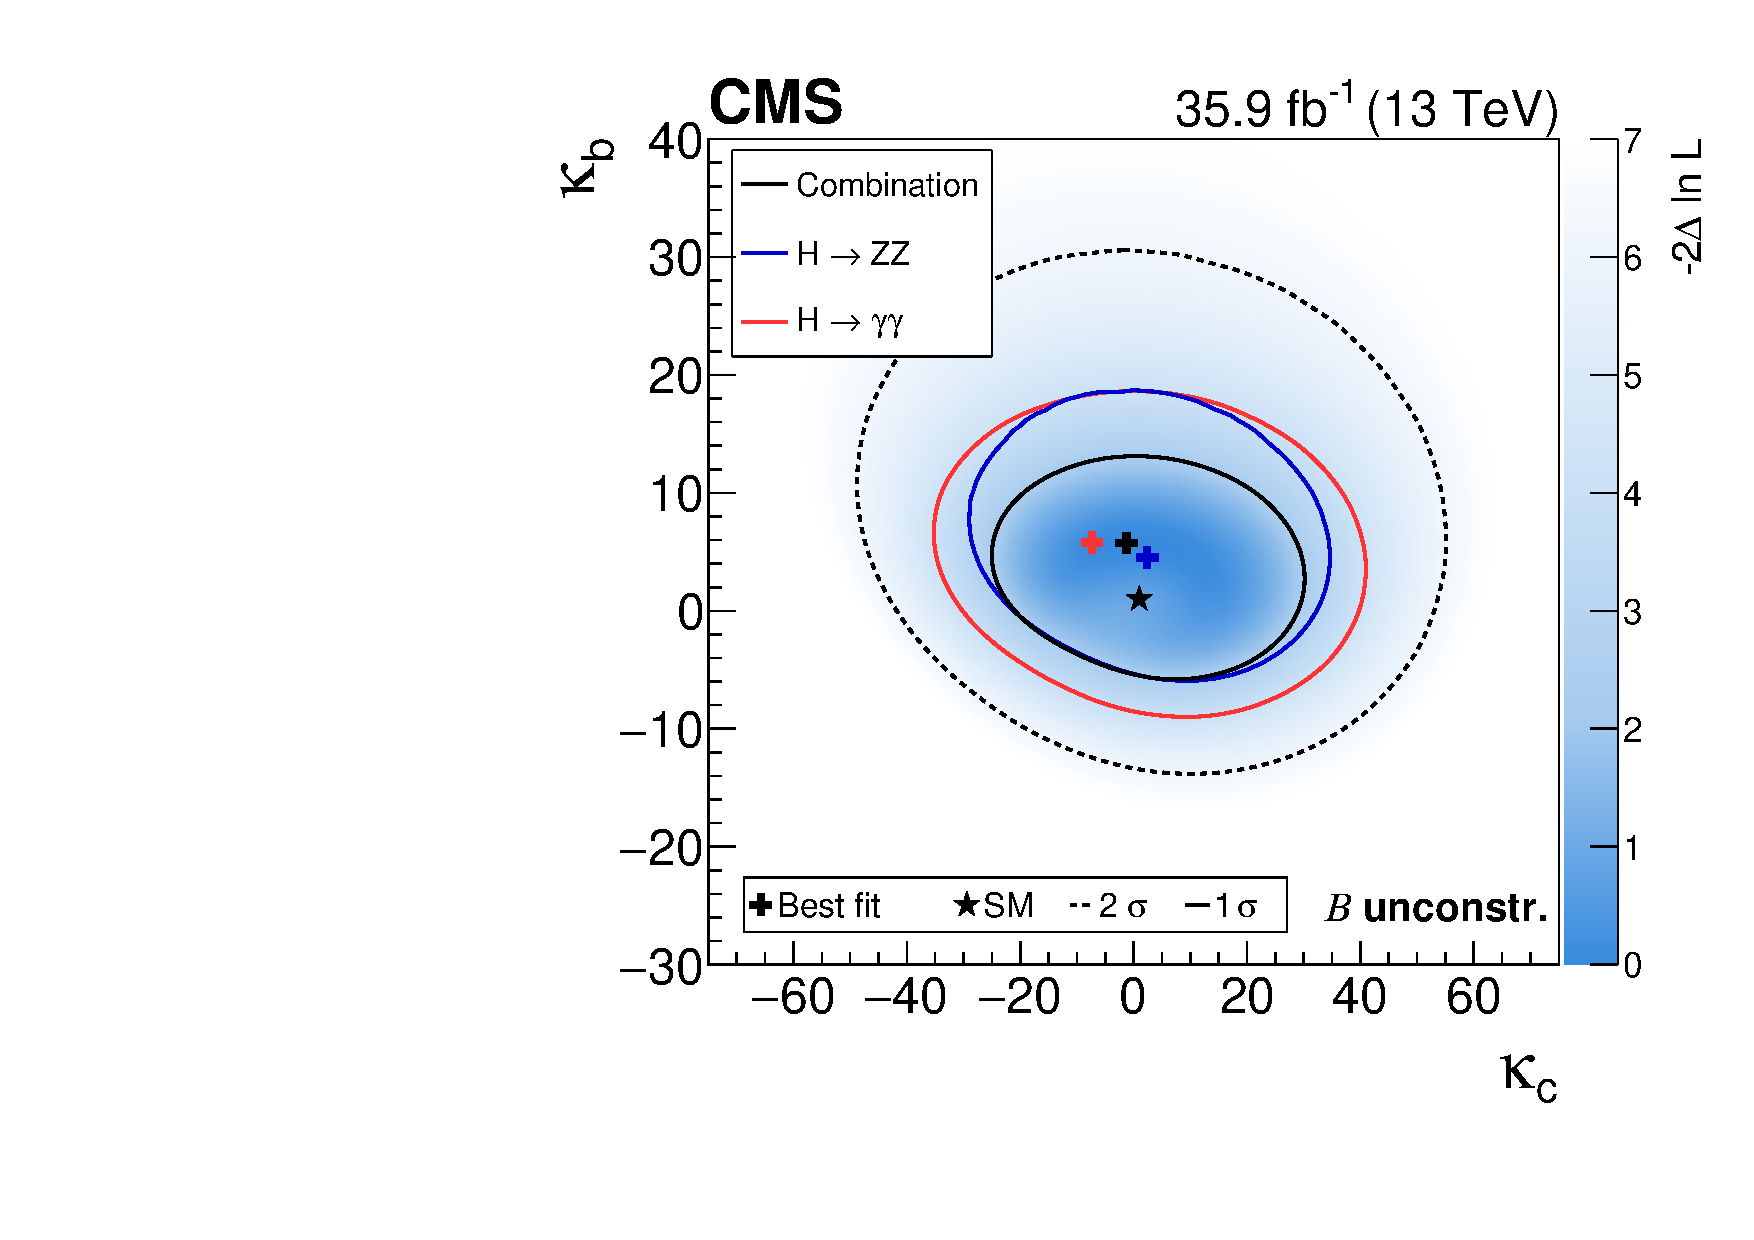
\includegraphics[width=0.49\linewidth]{img/interpretation/multicont_Yukawa_floatingBRs.pdf}        
        }
    % 
    \caption{
        Simultaneous fit to data for $\kappab$ and $\kappac$, assuming a coupling dependence of the branching fractions (left) and the branching fractions implemented as nuisance parameters with no prior constraint (right).
        % 
        The one standard deviation contour is drawn for the combination ($\hgg$ and $\hzz$), the $\hgg$ channel, and the $\hzz$ channel in black, red, and blue, respectively.
        % 
        For the combination the two standard deviation contour is drawn as a black dashed line, and the shading indicates the negative log-likelihood, with the scale shown on the right hand side of the plots.
        }
    \label{fig:kbkc}
  \end{center}
\end{figure}


For both scenarios of the branching fractions, scans are performed over each of the couplings individually while profiling the other, yielding the constraint on a single coupling.
% 
The scans are shown in Figs.~\ref{fig:kbkc-onedim-couplingdependent} for the coupling-dependent branching fractions.
% 
The `donut shape' stems mostly from constraints on the total width: At equal radii along the center of the circular band, $\sigma_\text{incl} \times \BRgamgam$ and $\sigma_\text{incl} \times \BRZZ$ are in agreement with the data, and deviating from the center of the circular band is thus excluded.
% 
The corresponding observed (expected) limits at 95\% CL are:
% 
\begin{linenomath*}
\begin{equation}
\label{eq:kappasensitivity}
\begin{array}{c}
\kappabLeftObserved < \kappab < \kappabRightObserved  \quad(\kappabLeftAsimov < \kappab < \kappabRightAsimov )  \,,
\\[8pt]
\kappacLeftObserved < \kappac < \kappacRightObserved \quad(\kappacLeftAsimov < \kappac < \kappacRightAsimov )
\,.
\end{array}
\end{equation}
\end{linenomath*}
% 
Likewise, for the unconstrained branching fractions the scans are shown in Figs.~\ref{fig:kbkc-onedim-couplingdependent}, and the corresponding observed (expected) limits at 95\% CL are:
% 
\begin{linenomath*}
\begin{equation}
\label{eq:kappasensitivity_floatingBRs}
\begin{array}{c}
\kappabLeftObservedFLOATINGBRS < \kappab < \kappabRightObservedFLOATINGBRS  \quad(\kappabLeftAsimovFLOATINGBRS < \kappab < \kappabRightAsimovFLOATINGBRS )  \,,
\\[8pt]
\kappacLeftObservedFLOATINGBRS < \kappac < \kappacRightObservedFLOATINGBRS \quad(\kappacLeftAsimovFLOATINGBRS < \kappac < \kappacRightAsimovFLOATINGBRS )
\,.
\end{array}
\end{equation}
\end{linenomath*}
% 
In the proof-of-concept study in Ref.~\cite{Bishara:2016jga}, the branching fractions were fixed to their SM expectation, and as such the results obtained up to now are not directly comparable to the ones found in Ref.~\cite{Bishara:2016jga}.
% 
If the branching fractions are fixed to their SM expectations, the one-dimensional scans yield the following expected limits at 95\% CL:
% 
\begin{linenomath*}
\begin{equation}
\label{eq:kappasensitivity_fixedSMBRs}
\begin{array}{c}
-3.5 < \kappab < 5.1  \,,
 \\[8pt]
-13 < \kappac < 15
\,.
\end{array}
\end{equation}
\end{linenomath*}
% 
These intervals are comparable to those in Ref.~\cite{Bishara:2016jga}, where $\kappac \in [ -16, 18 ]$ at 95\% CL, noting that the results here are based on a larger data set.
% 
The intervals obtained are competitive with the intervals from other direct search channels summarized in Section~\ref{sec:introduction}.


\begin{figure}[hbtp]
  \begin{center}
    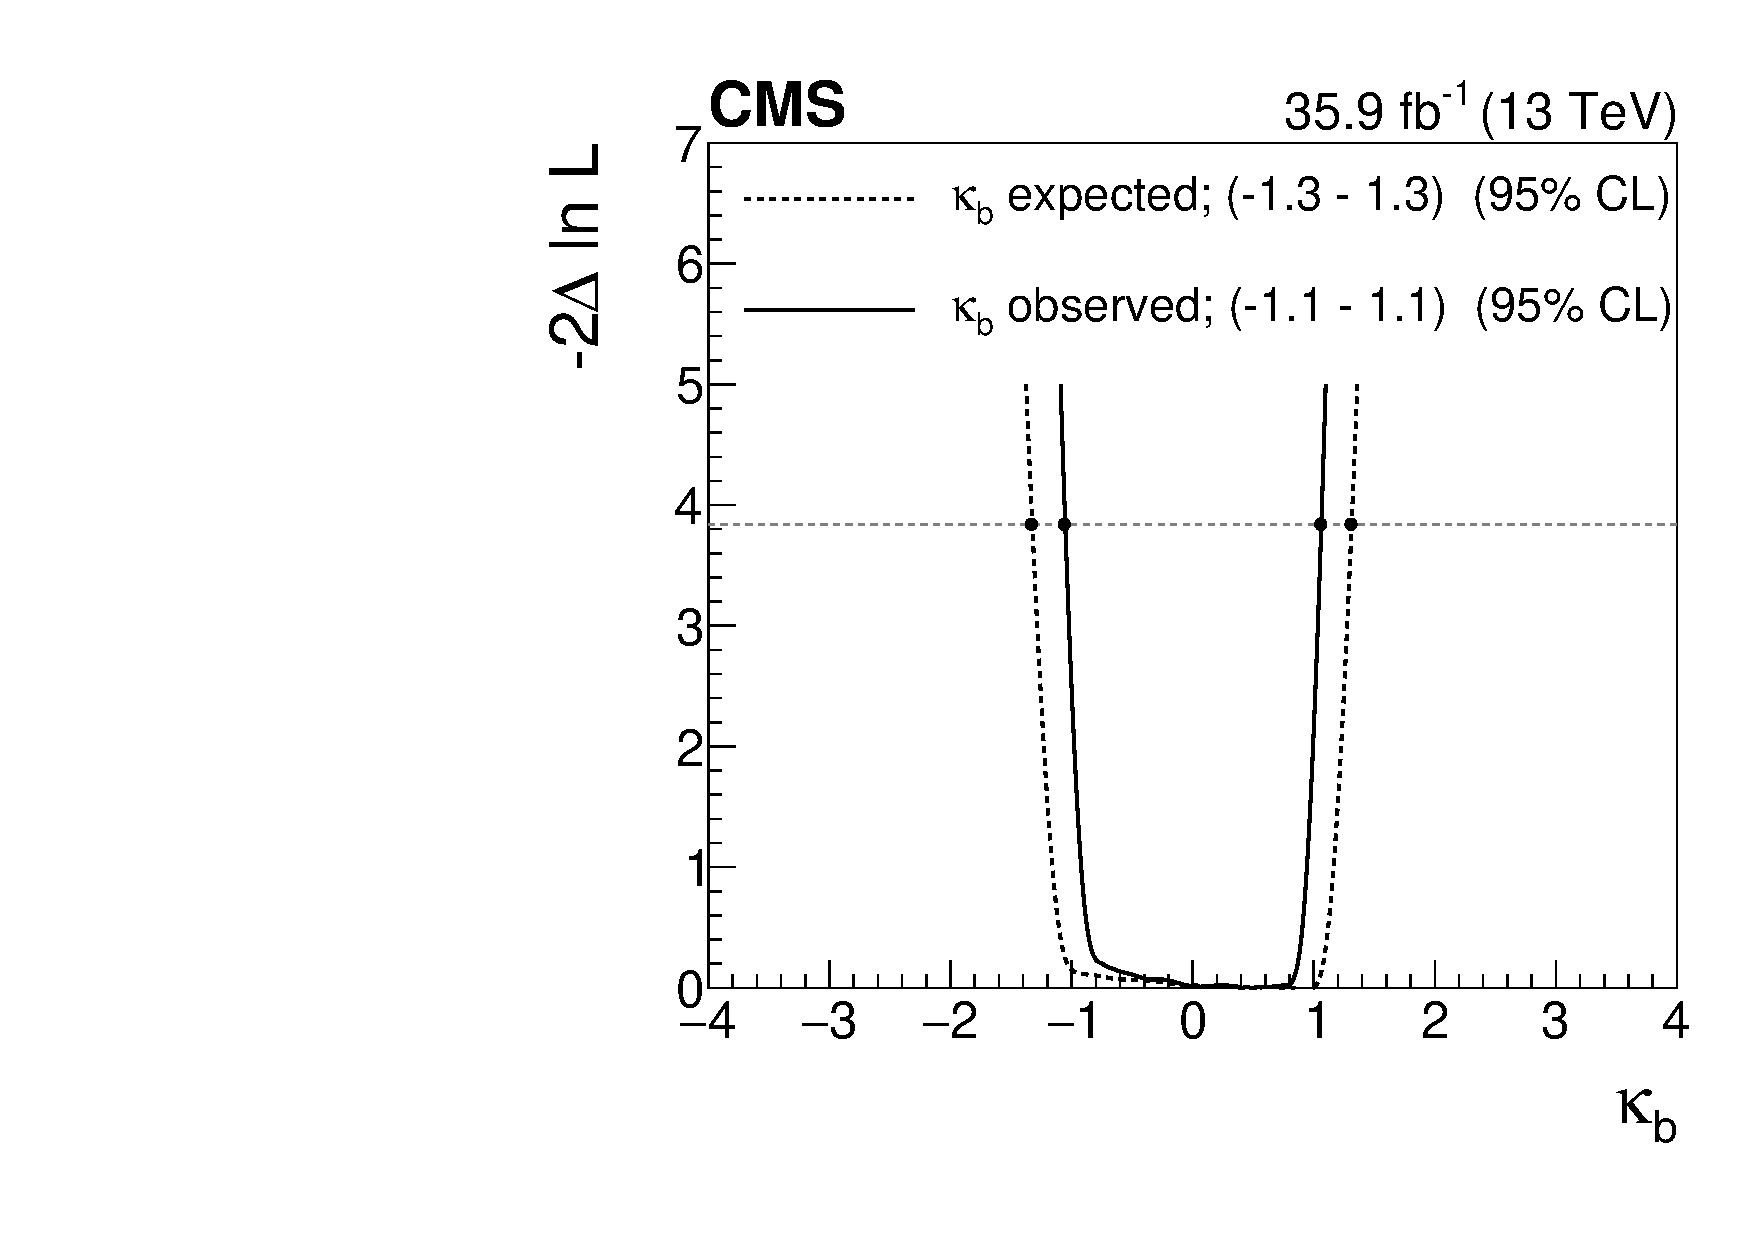
\includegraphics[width=0.49\linewidth]{img/interpretation/onekappascan_kbkc_couplingdependentBRs_kappab.pdf}
    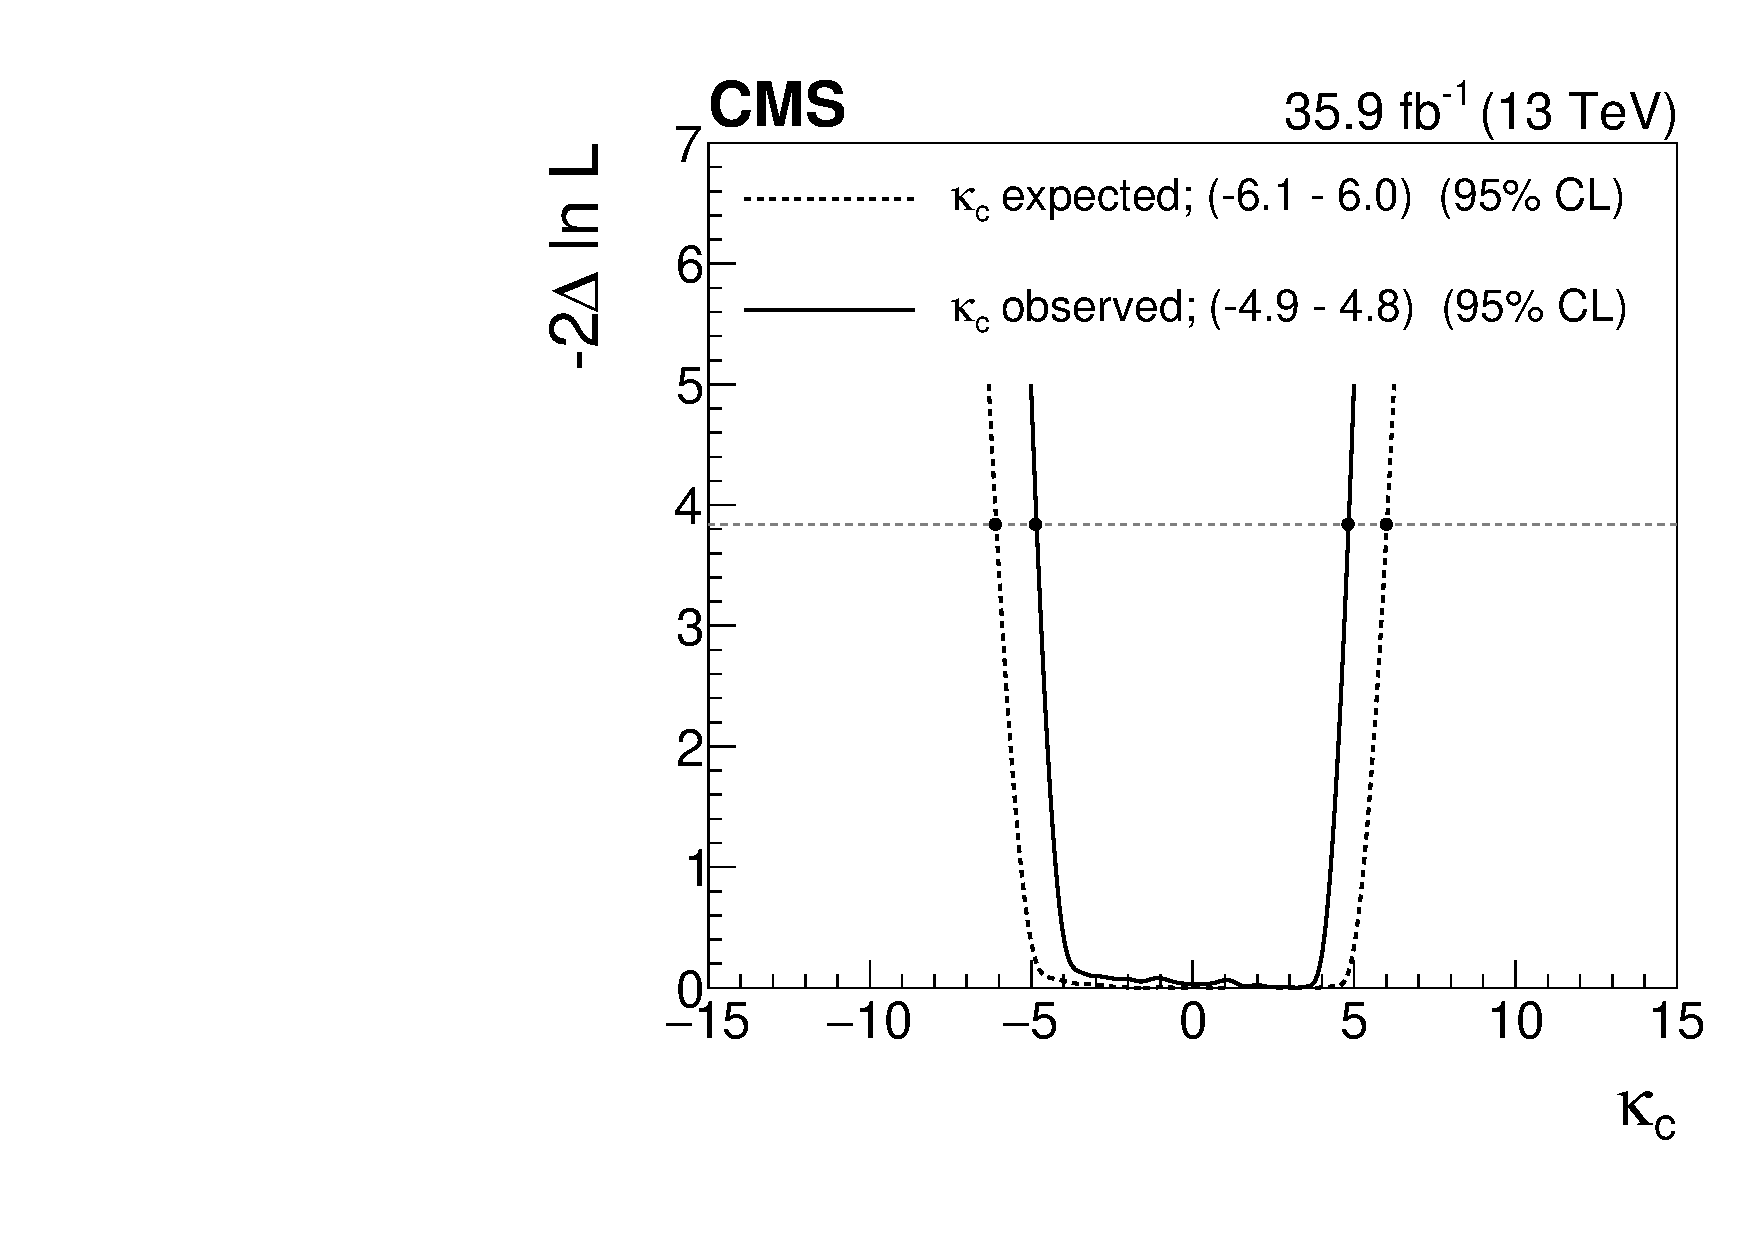
\includegraphics[width=0.49\linewidth]{img/interpretation/onekappascan_kbkc_couplingdependentBRs_kappac.pdf}
    \caption{
        Likelihood scan of $\kappab$ while profiling $\kappac$ (left), and of $\kappac$ while profiling $\kappab$ (right).
        % 
        The filled markers indicate the limits at 95\% CL.
        % 
        The branching fractions are considered dependent on the values of the couplings.
        }
    \label{fig:kbkc-onedim-couplingdependent}
  \end{center}
\end{figure}

\begin{figure}[hbtp]
  \begin{center}
    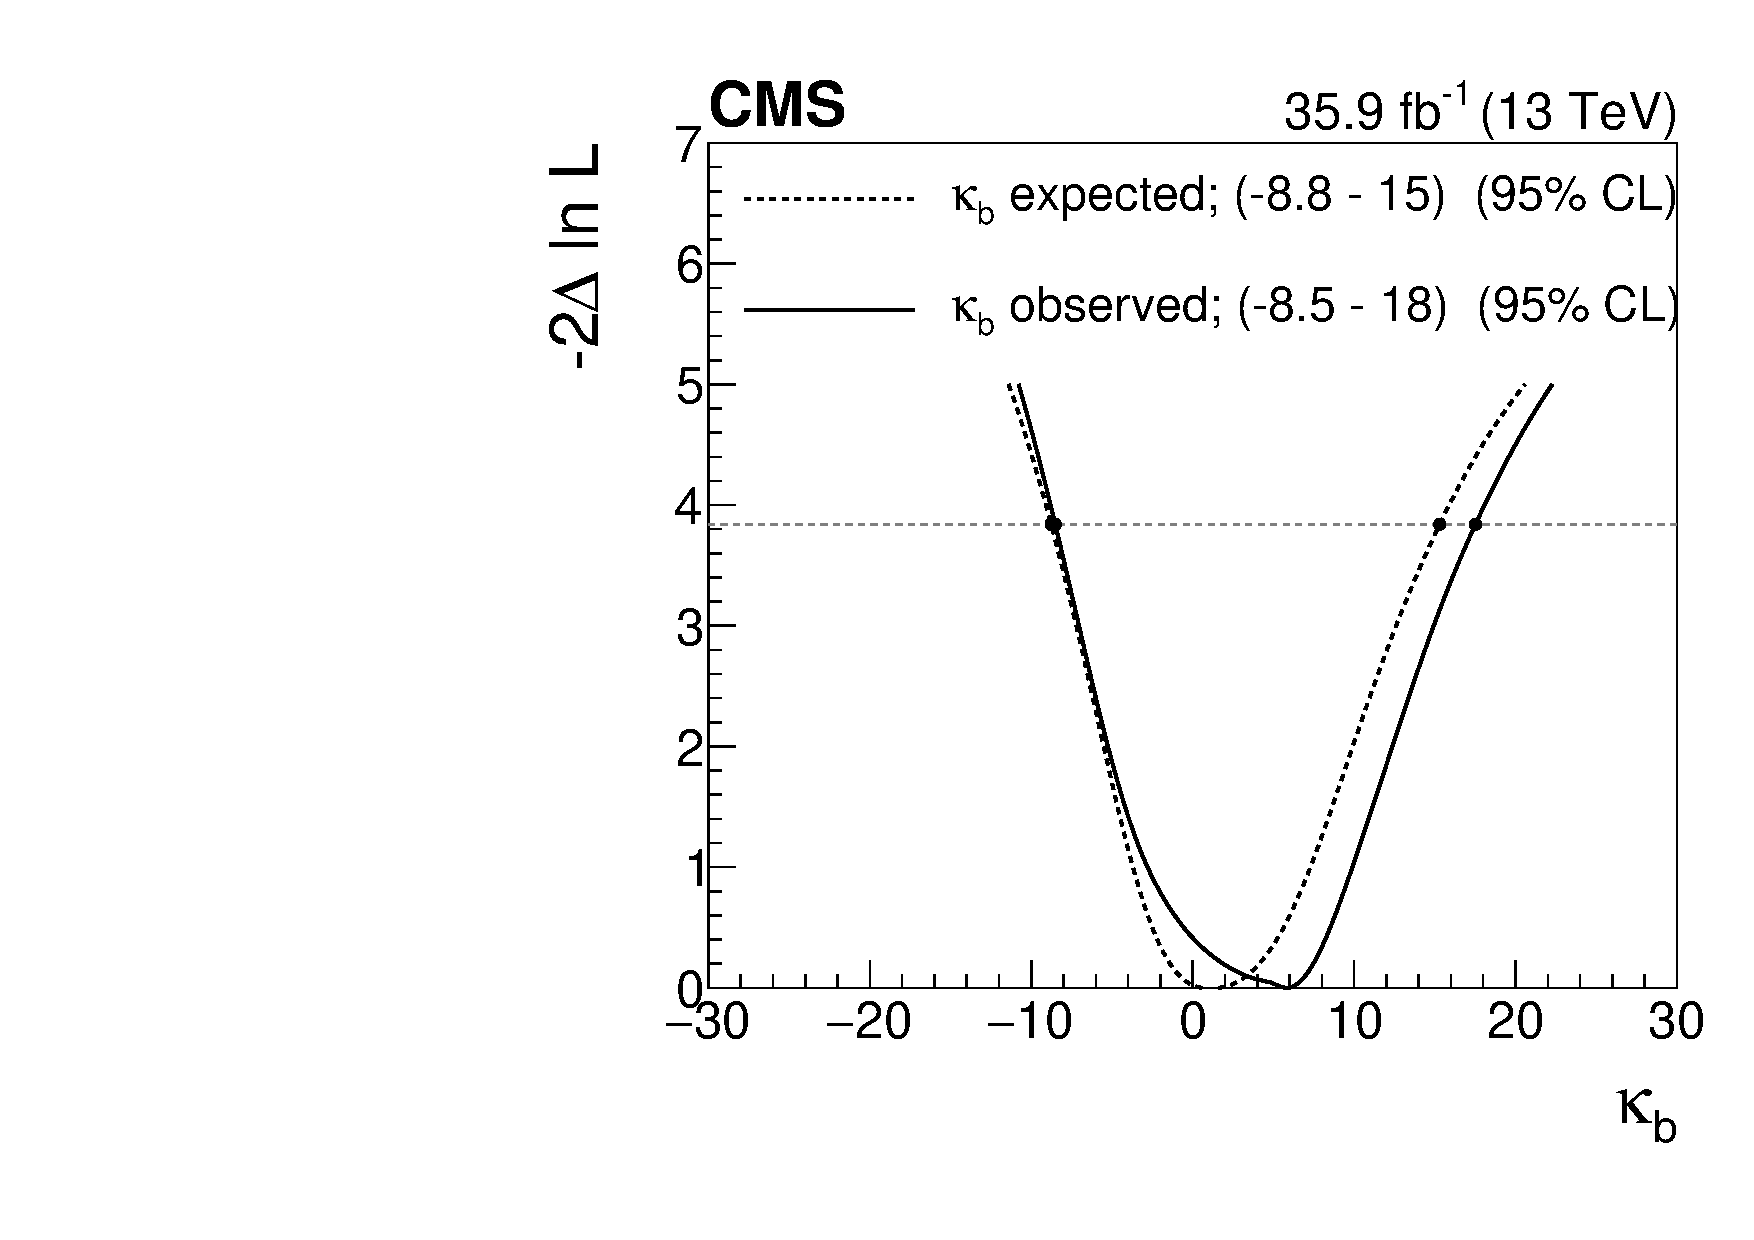
\includegraphics[width=0.49\linewidth]{img/interpretation/onekappascan_kbkc_floatingBRs_kappab.pdf}
    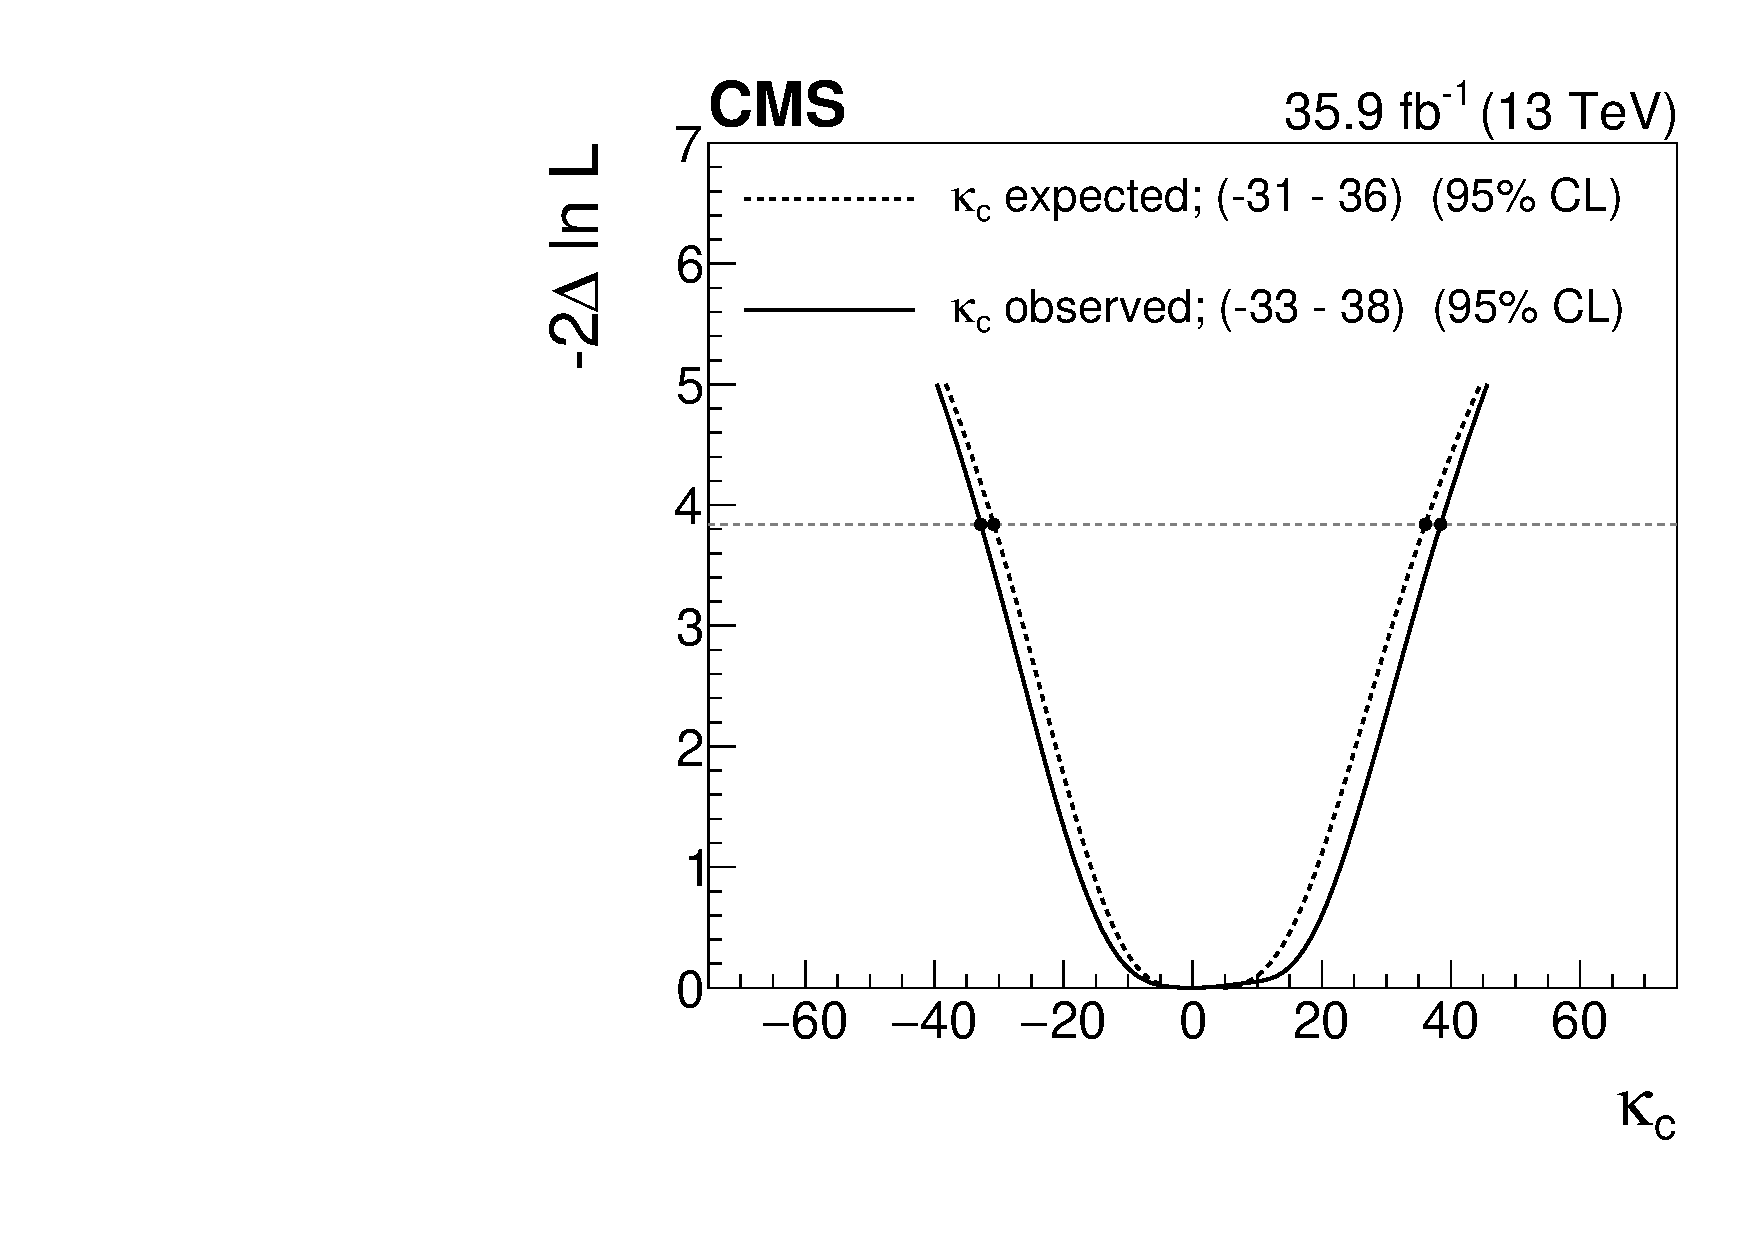
\includegraphics[width=0.49\linewidth]{img/interpretation/onekappascan_kbkc_floatingBRs_kappac.pdf}
    \caption{
        Likelihood scan of $\kappab$ while profiling $\kappac$ (left), and of $\kappac$ while profiling $\kappab$ (right).
        % 
        The filled markers indicate the limits at 95\% CL.
        % 
        The branching fractions are implemented as nuisance parameters with no prior constraint.
        }
    \label{fig:kbkc-onedim-floatingbrs}
  \end{center}
\end{figure}




